% \chapter{The Diversity-Quality Tradeoff and Its Impact on Generated Text Quality and Detectability}
\chapter{Measuring Generated Text Qualitiy and the Diversity-Quality Tradeoff}
\label{chap:decoding}

\section{Motivation}
It turns out that choosing the choice of decoding strategy (see Section \TODO{}) has a huge impact on the quality of the text that gets generated with a neural language model.
Search-based decoding strategies which optimize for choosing the mostly likely overall sequence end up producing text which is much less diverse than text a human writer would produce.
This may be tolerable for applications where diversity isn't strictly needed, such as machine translation, but it is problematic for applications where there are many valid ways to continue a prompt.
In this chapter, we present investigations of how the choice of decoding startegy creates a trade-off between the human-assessed quality of generated text and the amount of lexical diversity present in said text.

In Section \ref{section:dediv}, we consider search-based decoding strategies, focusing especially on diversity-promoting modifications of beam search.
We compared several methods which had previously never been compared with each other, and we showed that none of these diversity-promoting methods improve diversity without serious cost to generation quality.
No method outperformed the others on both diversity and quality.

In Section \ref{section:detection}, we focus on probabalistic generation methods which randomly sample a next word using the distribution predicted by the language model.
The simplest strategy is to sample directly from the predicted distribution.
However, when many low-likelihood words cumulatively contain quite a bit of probability mass, choosing one of these words can lead to odd or contradictory phrases and semantic errors.
Humans readers are quick to notice these types of errors.
Thus, more commonly, methods are used that reduce the entropy of the distribution before sampling, which improves generation quality at the cost of diversity.
We show that humans have a hard type identifying that text is machine-generated when sampling is heavily restricted to only high-likelihood words.

% \section{Definition and Measurement of Diversity}
\section{Terminology}
\subsection{Diversity}
The term ``diversity'' has been used in the language model literature to refer to a diverse set of properties.
Some use it as a synonym for sentence interestingness or unlikeliness \citep{tatsunori2019unifying}.
Others consider diversity a measure of how different two or more sentences are from each other \citep{vijayakumar2016diverse,gimpel2013systematic}.
In some framings, diversity is measured across a set of generations coming from the same prompt.
Given a particular prompt or input, the goal is to measure the breadth of possible generations the model will produce \citep{mayhew2020simultaneous}.
Diversity can also be measured as a corpus-level: given all the sentences generated by the model for all prompts, what is the overall lexical diversity \TODO{citation}?

In Section \ref{section:dediv}, we define diversity as the ability of a generative method to create a set of possible outputs that are each valid given a particular input but vary as widely as possible in terms of word choice, topic, and meaning.
We also use human evaluation to measure generation interestingness.
In Section \ref{section:detection}, we consider decoder-only language models, where no additional input is conditioned on.
In this setting, we instead consider corpus-level diversity across all the model's generations.
In both sections, diversity of a set of model generations is automatically measured using distinct-$n$, the number of unique $n$-grams within the set divided by the total number of $n$-grams.

\subsection{Quality}
``Quality'' is also a difficult property to define.
When measured in downstream applications, it can be quantified as how many times a user interactions with the generative system (for example, the number of conversation turns with a dialog system) before losing interest.
It can also be evaluated directly by asking a human rater, "how good is this text?", though definitions of ``good'' vary widely across the literature \TODO{add citation}.

To some extent, quality can also be measured automatically.
In tasks with a clear goal, like machine translation or summarization, one can compare the generation against a gold standard.
Generally, quality is strongly associated with fluency, and in \TODO{citation} we show that up until a point, the lower perplexity text is assigned by a language model, the more fluent it is.

Sections \ref{section:dediv} and \ref{section:detection} take quite different approaches to measuring generation quality.
In \ref{section:dediv}, we consider a dialog model, and ask humans to assess the quality of model responses on three axes: fluency, adequacy, and interestingness.
In  \ref{section:detection}, we propose a novel method for assessing generation quality based on the premise that humans (or a trained discriminator) ought to have a hard time distinguishing between real human-written text and model outputs when the model outputs text that is high-quality.

\section{Diversity-Promoting Search-Based Decoding Methods}
\label{section:dediv}
\subsection{Introduction}
In 2018, state-of-the-art neural language models were based on recurrent neural networks, such as LSTMs, that struggled to generate sequences that were both long and high-quality.
However, these models were beginning to have huge success over statistical techniques in natural language processing tasks such as machine translation \cite{sutskever2014sequence,Luong2015EffectiveAT}, text summarization \cite{Nallapati2016AbstractiveTS}, and dialog systems \cite{Vinyals2015ANC}.

At the time, the standard convention for generation was to try to generate the most likely overall sequence from the language model.
This approach made a lot of sense in machine translation, where generating one correct translation was more important than generating diverse translation.
Since computing the overall most likely output sequence is intractable, early work in neural machine translation found that beam search was an effective strategy to heuristically sample sufficiently likely sequences from these probabilistic models \cite{sutskever2014sequence}.
However, as neural language models came to be applied increasingly to open-ended tasks, beam search was found to be ill-suited to generating a set of diverse candidate sequences; this is because candidates outputted from a large-scale beam search often only differ by punctuation and minor morphological variations \cite{li2016mutual}.

There are a number of reasons why it is desirable to produce a set of diverse candidate outputs for a given input.
For example, in collaborative story generation, the system makes suggestions to a user for what they should write next \cite{clark2018creative}.
In these settings, it would be beneficial to show the user multiple different ways to continue their story.
In image captioning, any one sentence-long caption is probably missing some information about the image.
\citet{krause2017hierarchical} show how a set of diverse sentence-length image captions can be transformed into an entire paragraph about the image.
Lastly, in applications that involve reranking candidate sequences, the reranking algorithms are more effective when the input sequences are diverse.
Reranking diverse candidates has been shown to improve results in both open dialog and machine translation \cite{li2016diversity,li2016mutual,gimpel2013systematic}. 
Furthermore, in open-ended dialog, the use of reranking to personalize a model's responses for each user is a promising research direction \cite{Choudhary2017DomainAN}.

With these sorts of applications in mind, a variety of alternatives and extensions to beam search were proposed which sought to produce a set of diverse candidate responses instead of a single high likelihood one \cite{li2016diversity,vijayakumar2016diverse,kulikov2018importance,tam2019clustered}.
Many of these approaches show marked improvement in diversity over standard beam search across a variety of generative tasks.
However, as of 2018, there had been little attempt to compare and evaluate these strategies against each other on any single task.

In this sub-chapter, we survey methods for promoting diversity during decoding in order to systematically investigate the relationship between diversity and perceived quality of output sequences.
We focus on conditional language models--models that are trained to map from some input, perhaps an image or some text, to a target sequence.
In addition to standard beam search and greedy random sampling, we compare several recently proposed modifications to both methods.
We present a detailed comparison of existing diverse decoding strategies on two tasks: open-ended dialog and image captioning, and recommendations for a diverse decoding strategy.

\subsection{Diverse Decoding Strategies}
There are many ways to decode text from a conditional language model.
Let $\by$ represent the sequence of tokens for the target sequence ($\by = y_1 \ldots y_n$) and $\bx$ represent the input (which may be another token sequence, or, in the case of image captioning, an image).
Most decoding strategies strive to find the most likely overall sequence, i.e. pick a $\mathbf{\hat{y}}$ such that:\footnote{The formulation we are using here is slightly different than Section \TODO{}, in that we use $\by$ and $\hat{\by}$ to refer to sequence of tokens, rather than framing in terms of a sequence of embedding vectors.}
\[
    \mathbf{\hat{y}} = \arg\max_{\mathbf{y}}{ P(\mathbf{y} | \mathbf{x})} = \arg\max_{\mathbf{y}}{\prod_{t=1}^{N} {P(y_t \mid y_{<t}, \mathbf{x})}}
\]
In practice, this can't be computed exactly, no sub-exponential algorithm exists for find the optimal decoded sequence, and thus the field instead use approximations.

Beam search approximates finding the most likely sequence by performing breadth-first search over a restricted search space.
At every step of decoding, the method keeps track of $b$ partial hypotheses.
The next set of partial hypotheses are chosen by expanding every path from the existing set of $b$ hypotheses, and then choosing the $b$ with the highest scores.
If the goal is to approximate finding the most likely over-all sequence, the log-likelihood of the partial sequence is used as the scoring function.
Algorithm \ref{alg:beam-search-inference} gives an overview of the beam search algorithm. 

\begin{algorithm}
\caption{Beam Search Inference}
\label{alg:beam-search-inference}

\begin{algorithmic}[1]
\Procedure{Beam Search}{}
\State $B \gets \{SOS\}$
\State $k \gets $ BeamWidth
\State $out \gets k$-best output list
\While{$|out| < k$}
    \State $front \gets \text{remove all nodes from} B$
    \For{$w \in front$}
    \State $succ \gets w$'s $k$-best successors
    \For{$s \in succ$}
    \If{$s == EOS$}
        \State $out \gets out \cup \{s\}$
    \Else
        \State $B \gets B \cup \{s\}$
    \EndIf
    \EndFor
    \EndFor
    \State Sort $B$
    \If{$|B| > k$}
        \State Prune $B$ to $k$-best successors
    \EndIf
\EndWhile

\Return out
\EndProcedure
\end{algorithmic}
\end{algorithm}

Since beam search only explores a limited portion of the overall search space, it tends to yield multiple variants of the same high-likelihood sequence, sequences that often only differ in punctuation and minor morphological changes \cite{li2016mutual}.  
Therefore, standard beam search is not ideal for producing diverse outputs.
In this section, we will discuss a variety of methods that have been developed recently to eliminate redundancy during decoding and generate a wider range of candidate outputs.

\paragraph{Noisy Parallel Approximate Decoding}\quad
Introduced by \citet{cho2016noisy}, NPAD is a technique than can be applied to any decoding setting.
The main idea is that diversity can be achieved more naturally by taking advantage of the continuous manifold on which neural nets embed language.
Instead of encouraging diversity by manipulating the probabilities outputted from the model, diverse outputs are instead produced by adding small amounts of noise to the hidden state of the decoder at each step.
The noise is randomly sampled from a normal distribution. The variance is gradually annealed from a starting $\sigma_0$ to 0 as decoding progresses (that is $\sigma_t = \frac{\sigma_0}{t}$) under the reasoning that uncertainty is greatest at the beginning of decoding.
NPAD can be used in conjunction with any decoding strategy; following the best results from the original paper, we show results using NPAD with beam search.

Extensions to NPAD have sought to learn the direction in which to manipulate the hidden states using an arbitrary decoding objective \cite{gu2017trainable}.
Since such objectives can be highly domain-specific, we do not evaluate this method.

\paragraph{Top-$g$ Capping}\quad
In beam search, it is often the case that one hypothesis $h$ is assigned a much higher probability than all other hypotheses, causing all hypotheses in the next step to have $h$ as their parent. Following \citet{li2016mutual} and \citet{li2016simple}, we add an additional constraint to standard beam search to encourage the model to choose options from diverse candidates.
At each step $t$, current hypotheses are grouped according to the parental hypothesis they come from.
After grouping candidates, only the top $g$ from each grouping are considered. The resulting $b \times g$ candidates are ranked, and the top $b$ are selected as hypotheses for the next beam step.

\paragraph{Hamming Diversity Reward}\quad
\citet{vijayakumar2016diverse} proposes adding an additional diversity-promoting term, $\theta$, to the log-likelihood before reranking.
This term measures how different a candidate hypothesis $c^{(i)}_{\leq t}$ is from the partial hypotheses selected in the previous step. Let $\mathcal{H}_{t-1} = \{c^{(1)}_{\leq t-1}$, \ldots $c^{(b)}_{\leq t-1}\}$ be these partial hypotheses.
Then the beam search scoring function for the $i$th candidate at timestep $t$ becomes:
\begin{align*}
    \text{score}(c^{(i)}_{\leq t}) = \sum_{j=1}^t \big(\log P(c^{(i)}_j | c^{(i)}_{<j}, \textbf{x})\big) \\+ \lambda\theta(c^{(i)}_{\leq t}, \mathcal{H}_{t-1})
\end{align*}
where $\lambda$ is a tunable hyperparameter. \citet{vijayakumar2016diverse} try a variety of definitions for $\theta$, including embedding diversity and $n$-gram diversity, but they find that Hamming distance, the number of tokens in the candidate sequence which exist in the previously selected partial hypotheses, is most effective. We take the negative of the Hamming distance as $\theta$.

\paragraph{Iterative Beam Search}\quad
In an attempt to improve the size of the search space explored without sacrificing runtime, \citet{kulikov2018importance} propose an iterative beam search method.
Beam search is run many times, where the states explored by subsequent beam searches are restricted based on the intermediate states explored by previous iterations.
Formally, we can define the set of all partial hypotheses for beam search instance $i$ at time step $t$ as $\mathcal{H}_t^{(i)}$. From here, the search space explored by beam search instance $i$ can be expressed as $S_i = \cup_{t=1}^T \mathcal{H}_t^{(i)}$.
The $i$th beam search is prevented from generating any partial hypothesis that has previously been generated, that is, any hypothesis found in $S_{<i} = \cup_{i^{\prime}=0}^{i-1}S_{i^{\prime}}$.

The authors also attempt a soft inclusion criterion, where any states within $\epsilon$ Hamming distance from a previously explored state are also excluded. During the experimentation of \citet{kulikov2018importance}, however, the soft-inclusion was found to not be beneficial; thus, we only restrict exact matches of previous states in our implementation.
In practice, this means after the first beam search instance runs as normal, the first step of the second beam search instance will contain the $b$+1 to 2$b$-most likely starting tokens; this pattern holds for the third beam search instance, and so on.

\paragraph{Clustered Beam Search}\quad
Most recently, \citet{tam2019clustered} proposed a clustering-based beam search method to help condense and remove meaningless responses from chatbots.
Specifically, at each decoding step $t$, this method initially considers the top $2*b$ candidates. From there, each candidate sequence is embedded\footnote{We follow \citet{tam2019clustered} and used averaged GloVe word embeddings \cite{pennington2014glove}.}, and the embeddings are clustered into $c$ clusters using $K$-means. Finally, we take the top $\frac{b}{c}$ candidates from each cluster. Note that in the case any clusters have size less than $\frac{b}{c}$, we then include the highest-ranked candidates not found after clustering.

\paragraph{Clustering Post-Decoding (PDC)}
All the previous methods modified the decoding algorithm to encourage diversity.
However, it is also possible to encourage additional diversity post-hoc by sampling several generations and then choosing the most diverse one.
On the task of sentence simplification, after decoding using a large-scale diversity-promoting beam search (beam size 100), \citet{kriz2019complexity} then clustered similar sentences together to further increase the variety of simplifications from which to choose.
Document embeddings generated via Paragraph Vector \cite{Le2014distributed} were used as the sentence embeddings with which to perform $K$-means. 

In this work, we extend this post-decoding clustering idea in three key ways.
First, we make use of sentence-level embeddings which leverage the pre-trained language representations from the Bidirectional Encoder Representations from Transformers (BERT) \cite{devlin2018bert}.\footnote{BERT sentence-level embeddings were obtained using https://github.com/hanxiao/bert-as-service.}
Second, after clustering, \citet{kriz2019complexity} took the sentence closest to the centroid of each cluster as the representative candidate; we instead choose the highest-ranked candidate (according to log-likelihood) from each cluster to ensure the best candidates are still selected.
Finally, after performing standard $K$-means clustering, we found that it was often the case that some clusters contained large numbers of good candidates, while others contained very few candidates that are also either ungrammatical or otherwise inferior.
Thus, in our implementation, we remove clusters containing two or fewer sentences, and then sample a second candidate from each of the remaining clusters, prioritizing selecting candidates from larger clusters first.


\subsection{Experimental Setup}
We evaluate the decoding strategies described in the previous section under the following settings.
For each of the published beam search algorithms, we choose the hyperparameters that were found to be best in the original publications.\\

\small
\begin{tabular}{l|l}
    \toprule
    Method & Setting\\
    \midrule
    \multirow{2}{*}{RS} & Random sampling with temp = 0.5,\\
    & 0.7, 1.0, or 1.0 with top-10 capping.\\
    Standard BS & Standard beam search\\
    Top5Cap BS & Top-$g$ capping with $g=3$\\
    Iter5 BS & Iterative beam search with 5 iterations\\
    HamDiv0.8 BS & Hamming Diversity with $\lambda=0.8$\\
    Cluster5 BS & Clustered beam search with 5 clusters\\
    NPAD0.3 BS & Noisy Decoding with $\sigma_0=0.3$ \\
    \bottomrule
\end{tabular}
\normalsize
\\

For random sampling, we sample 10 outputs, and with beam-search based methods, we use a beam size of 10 to generate 10 outputs.
In addition, we show results from oversampling then filtering.
We use a beam size of 100 or generate 100 samples through random sampling, and then we select 10 from the 100, either through post-decoding clustering (PDC) or by taking the 10 candidates with highest likelihood. 

We examine these decoding strategies on two tasks: open ended dialog and image captioning.
For each task, we evaluate both the quality and diversity of the 10 outputs from each strategy.

\subsubsection{Open-ended Dialog Task}
In the dialog domain, we use an LSTM-based sequence-to-sequence (Seq2Seq) model implemented in the OpenNMT framework \cite{opennmt}.
We match the model architecture and training data of \citet{baheti2018generating}.
The Seq2Seq model has four layers each in the encoder and decoder, with hidden size 1000, and was trained on a cleaned version of OpenSubtitles \cite{tiedemann2009news} to predict the next utterance given the previous one.

Evaluation is performed on 100 prompts from the Cornell Movie Dialog Corpus~\cite{danescu2011chameleons}.
These prompts are a subset of the 1000 prompts used in \citet{baheti2018generating}, which were filtered using item response theory for discriminative power.

We report perplexity (PpL), averaged over \textit{all} the top 10 outputs for each example.\footnote{This differs from existing work which computes perplexity over only the top output for each example. For our task we are interested in the quality of all of the generated responses.} Since the quality of open-ended dialog is notoriously difficult to evaluate automatically, we ran a human evaluation task on Amazon Mechanical Turk where annotators were shown a prompt and 5 potential responses generated by any of our decoding methods.
Evaluators were asked to provide binary ratings on fluency, adequacy, and interestingness for each response. Overall, we collected 3 human judgments for each of the top ten responses for each of our decoding methods; in other words, we collected 3,000 judgments per method.
Figure \ref{TODO} show the instructions given to the human raters.

\begin{figure*}
    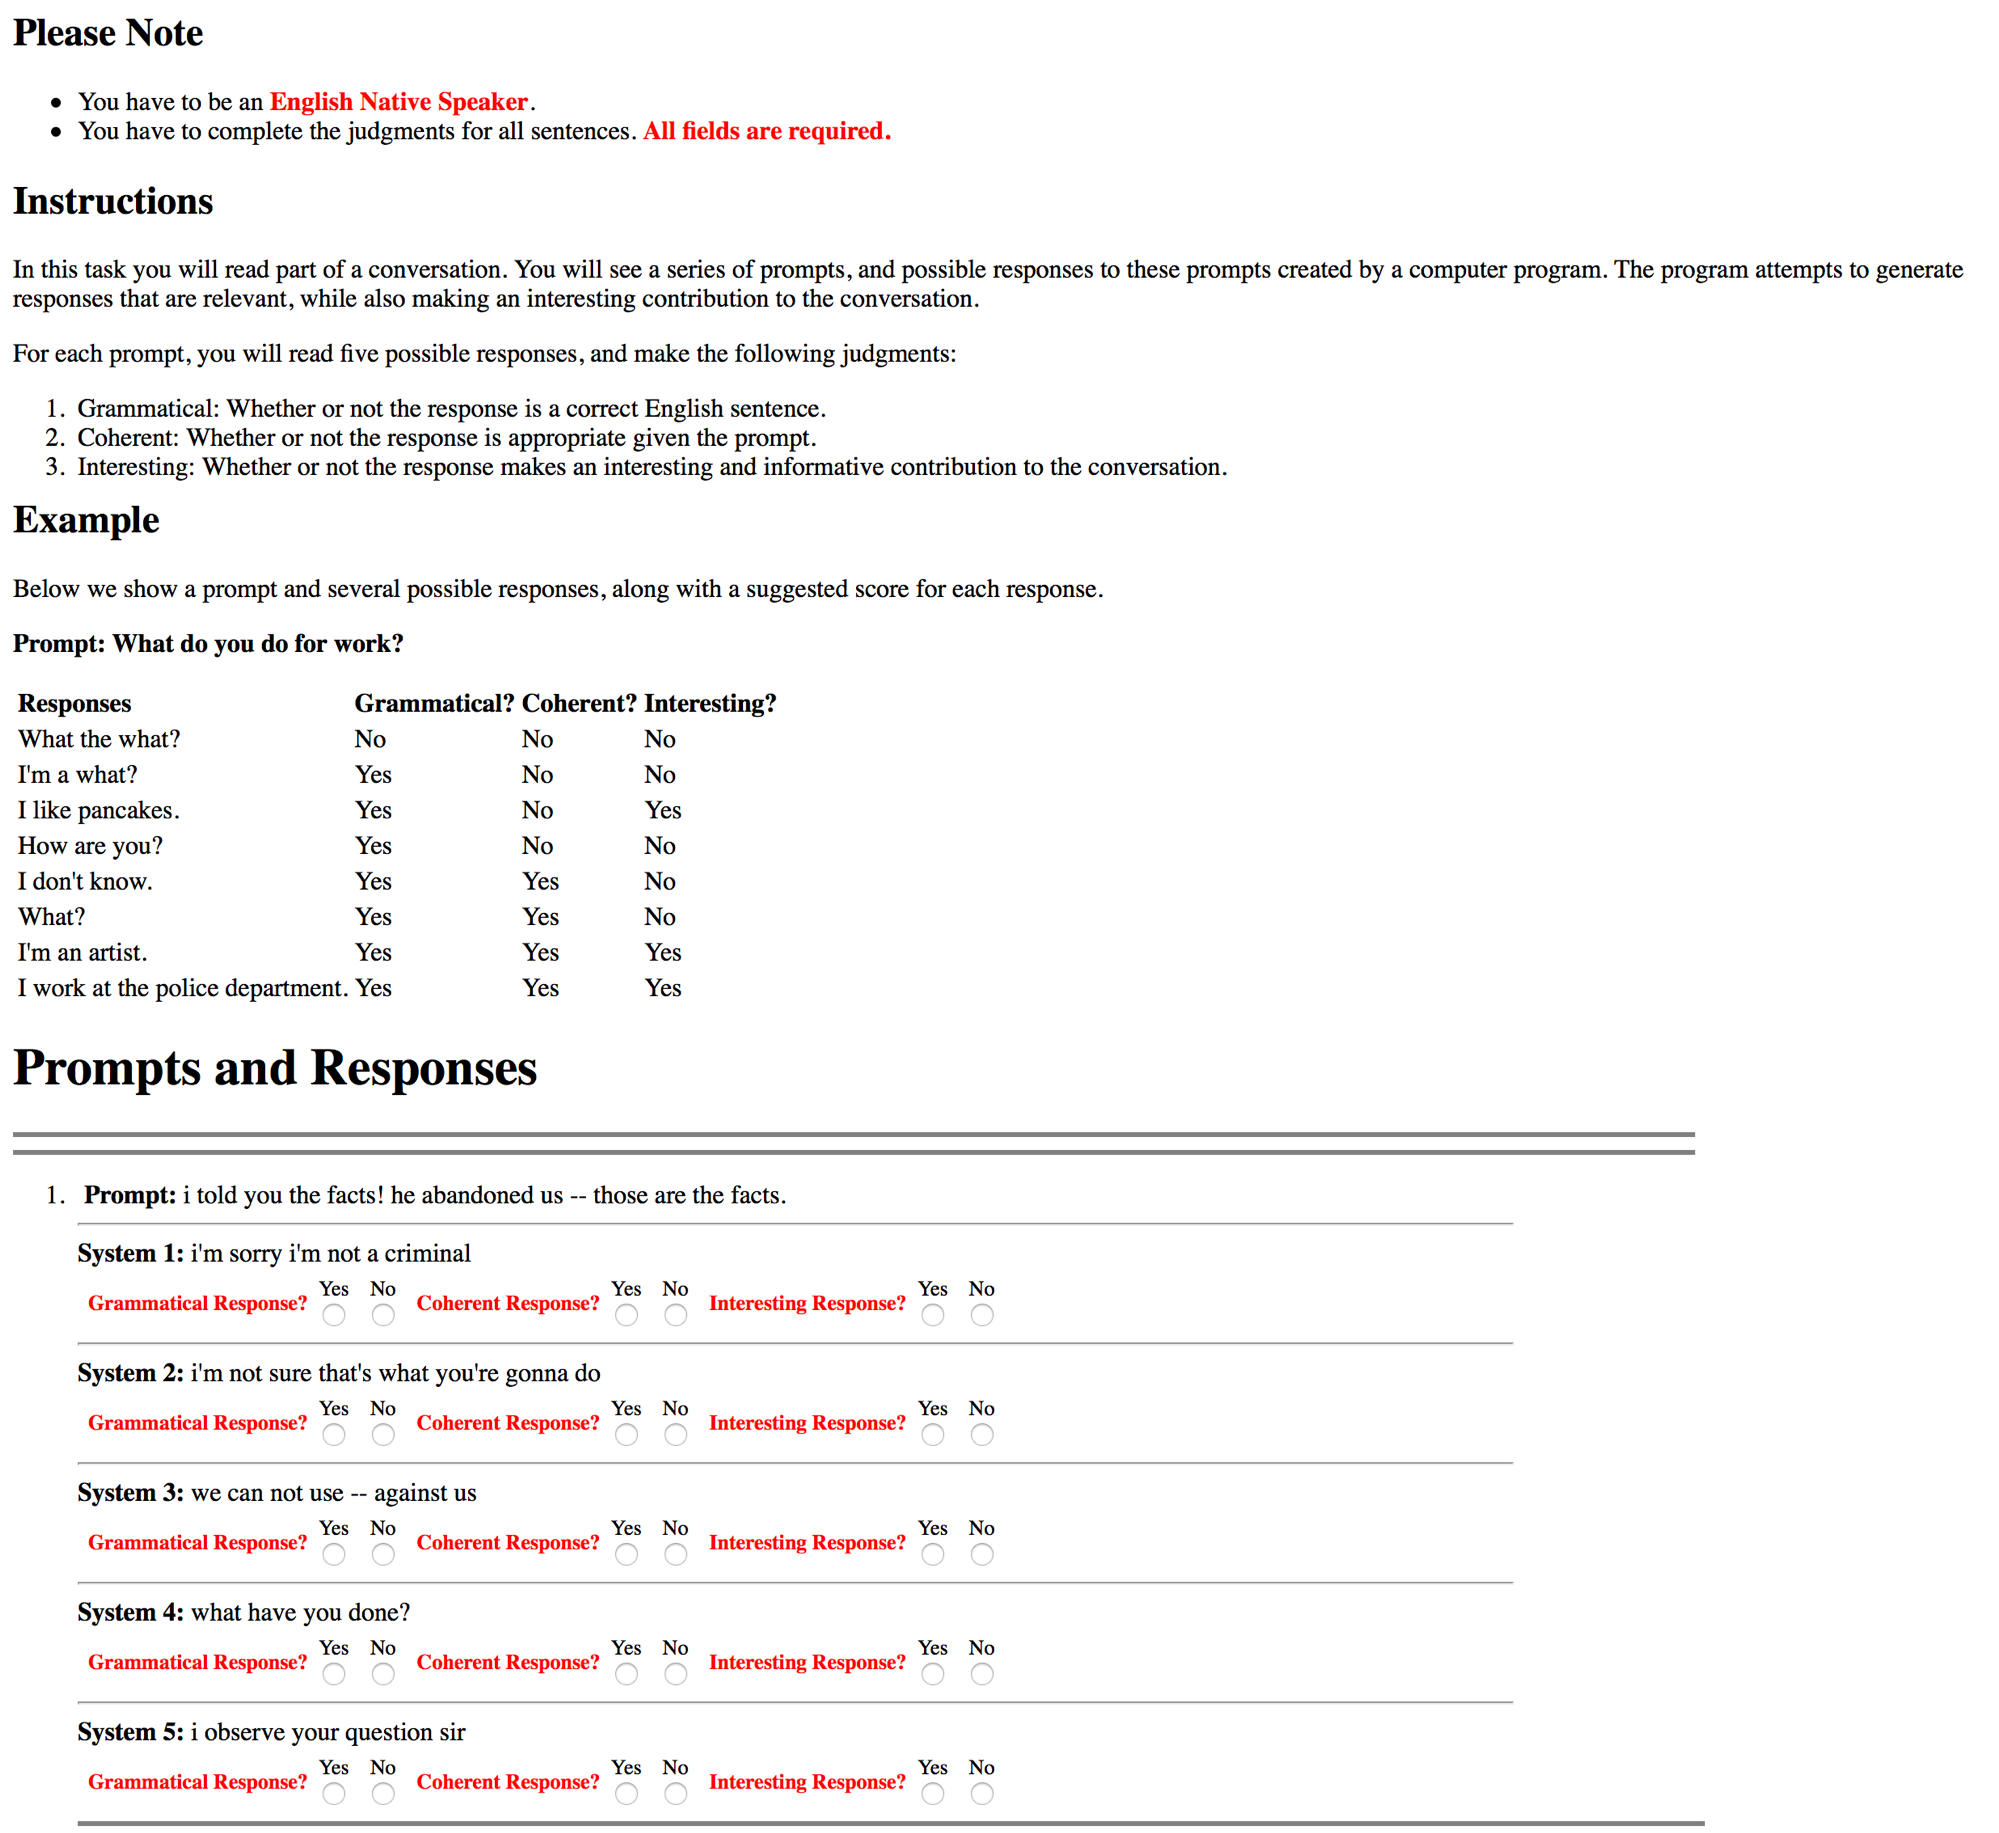
\includegraphics[width=\textwidth]{figures/dediv_mturk_example.png}
    \caption{The full instructions for our Amazon Mechanical Turk task to evaluate the quality of our dialog system responses.}
    \label{mturk_example}
\end{figure*}

\begin{table*}[t]
    \centering
    \tiny
    \setlength\tabcolsep{4pt} 
    \begin{tabular}{|lr||ccc||ccccc|} \hline
    
    \multicolumn{2}{|c||}{\textbf{Method}} & \textbf{Fluency} & \textbf{Adequacy} & \textbf{Interestingness} & \textbf{Ppl} & \textbf{Dist-1} & \textbf{Dist-2} & \textbf{Ent-2} & \textbf{Ent-4} \\ \hline\hline
    Reference & & 0.795 & 0.732 & 0.636 & -- & -- & -- & -- & -- \\ \hline\hline
    RS 0.7 &(sample 10) & \textbf{0.758} & 0.399 & \textbf{0.388} & 35.98 & 0.63 & 0.80 & 4.08 & 3.84 \\
    RS 1.0 &(sample10) & 0.550 & 0.303 & \td{0.386} & 67.99 & \textbf{0.74} & \textbf{0.87} & \textbf{4.35} & \textbf{4.08} \\
    RS 1.0,top10 &(sample 10) & \td{0.745} & \textbf{0.418} & \td{0.387} & \textbf{10.33} & 0.60 & 0.80 & 4.12 & 3.91 \\ \hline\hline
    Standard BS &(10 beams) & \textbf{0.950} & \textbf{0.621} & 0.336 & \textbf{4.01} & 0.37 & 0.45 & 3.16 & 3.01 \\
    Top3Cap BS &(10 beams)& \td{0.942} & 0.603 & 0.346 & 4.03 & 0.37 & 0.46 & 3.17 & 3.03 \\
    Iter5 BS &(10 beams)& 0.903 & 0.520 & 0.335 & 5.42 & \textbf{0.62} & \textbf{0.74} & \textbf{3.68} & \textbf{3.25} \\
    HamDiv0.8 BS &(10 beams)& 0.923 & 0.599 & \td{0.366} & 4.56 & 0.33 & 0.37 & 3.08 & 3.00 \\
    Cluster5 BS &(10 beams)& 0.936 & 0.582 & \textbf{0.381} & 4.23 & 0.39 & 0.46 & 3.24 & 3.06 \\
    NPAD0.3 BS &(10 beams) & \td{0.942} & \td{0.604} & 0.335 & 4.05 & 0.36 & 0.44 & 3.13 & 2.99 \\ \hline\hline
    RS 1.0,top10 &(sample 100, rank) & \textbf{0.922} & \textbf{0.548} & 0.347 & \textbf{5.10} & 0.52 & 0.68 & 3.54 & 3.18 \\
    RS 1.0,top10 &(sample 100, PDC) & 0.852 & 0.494 & \textbf{0.372} & 6.96 & \textbf{0.63} & \textbf{0.76} & \textbf{3.74} & \textbf{3.27} \\ \hline\hline
    Standard BS &(100 beams, rank) & \textbf{0.964} & \textbf{0.611} & \td{0.332} & \textbf{4.01} & 0.44 & 0.61 & 3.33 & 3.05 \\
    Standard BS &(100 beams, PDC) & 0.944 & 0.599 & \textbf{0.346} & 4.42 & \textbf{0.57} & \textbf{0.70} & \textbf{3.59} & \textbf{3.21} \\ \hline
    \end{tabular}

    \caption{
    Results on 100 dialog prompts.
    The first row shows the mean human ratings of the single reference response available for each prompt.
    The next three rows show results for random sampling, with 10 samples drawn per prompt. The next six rows are variants of beam search using beam size 10.
    The last four rows use random sampling or standard beam search to generate 100 outputs, then filter down to 10 outputs either through ranking by log-likelihood or by performing post-decoding clustering (PDC).
    In each section, the highest value is bolded, and statistical ties are marked \textdagger.}
    \label{tab:results_no_cluster}
\end{table*}

\begin{table*}
    \small
    \centering
\begin{tabular}{|lr||ccc||cccc|}
\hline
 & & \multicolumn{3}{c||}{\textbf{SPICE}} & & & & \\
\multicolumn{2}{|c||}{\textbf{Method}} & \textbf{Mean} & \textbf{@1} & \textbf{@10} & \textbf{Dist-1} & \textbf{Dist-2} & \textbf{Ent-2} & \textbf{Ent-4}  \\
\hline\hline
RS 0.7 &(sample10)               & \textbf{0.170} & \textbf{0.192} & \textbf{0.278} & 0.31 & 0.52 & 3.67 & 4.00 \\
RS 1.0 &(sample10)               & 0.133 & 0.167 & 0.247 & \textbf{0.44} & \textbf{0.71} & \textbf{4.17} & \textbf{4.26} \\
RS 1.0,top10 &(sample10)         & 0.159 & 0.183 & 0.272 & 0.33 & 0.59 & 3.90 & 4.17 \\
\hline \hline
Standard BS &(10 beams)               & 0.194 & 0.193 & 0.283 & 0.18 & 0.26 & 2.94 & 3.18 \\
Top3Cap BS &(10 beams)                & \textbf{0.195} & \textbf{0.196} & 0.282 & 0.17 & 0.26 & 2.93 & 3.17 \\
HamDiv0.8 BS &(10 beams)              & 0.194 & 0.194 & 0.282 & 0.18 & 0.27 & 2.98 & 3.19 \\
Cluster5 BS &(10 beams)               & 0.191 & 0.194 & \textbf{0.285} & \textbf{0.19} & \textbf{0.28} & \textbf{3.04} & \textbf{3.25} \\
NPAD0.3 BS &(10 beams)                & 0.191 & 0.192 & 0.280 & 0.18 & 0.26 & 2.94 & 3.17 \\
\hline \hline
RS 1.0,top10 &(sample100, rank)  & \textbf{0.182} & \textbf{0.188} & \textbf{0.284} & 0.25 & 0.41 & 3.31 & 3.64 \\
RS 1.0,top10 &(sample100, PDC)   & 0.169 & \textbf{0.188} & 0.282 & \textbf{0.31} & \textbf{0.52} & \textbf{3.62} & \textbf{3.91} \\
\hline \hline
Standard BS &(100 beams, rank)        & \textbf{0.188} & 0.190 & 0.279 & 0.20 & 0.31 & 3.04 & 3.32 \\
Standard BS &(100 beams, PDC)         & 0.186 & \textbf{0.192} & \textbf{0.288} & \textbf{0.24} & \textbf{0.38} & \textbf{3.25} & \textbf{3.57} \\
\hline
\end{tabular}
\caption{Image captioning results for selected random sampling and beam search methods. SPICE@1 measures the SPICE score of the most likely caption. SPICE@10 is the maximum score across the 10 candidates generated by each method. Mean SPICE is the mean score over all 10 candidates. In each section, the best value is bolded.}
\label{tab:image_captioning}
\end{table*}

\subsubsection{Image Captioning Task}
For image captioning, we use a state-of-the-art model introduced in \citet{anderson2018bottom}.
We take advantage of \citet{Luo2017}'s open-source implementation and released model parameters trained on MSCOCO \cite{lin2014microsoft}.
We evaluate on a test set containing 5000 images.

We report Semantic Propositional Image Caption Evaluation (SPICE) scores, an automatic evaluation metric that has been shown to correlate well with human judgments of quality\citep{Anderson2016SPICE}. 
SPICE measures how well the semantic scene graph induced by the proposed caption matches one induced by the ground truth.
In addition to computing SPICE on the top-scoring caption (SPICE@1), we follow \citet{vijayakumar2016diverse} in reporting Oracle SPICE@10 scores.
This is done to show the upper bound on the potential impact diversity can have.
We also compute the mean SPICE score across all of the candidate captions for an image.
Unlike SPICE@1 and SPICE@10, this metric shows the overall quality of \textit{all}
of the candidate captions, which is useful to know for applications that combine diverse candidate output sequences \cite{krause2017hierarchical}.

\subsubsection{Evaluating Diversity}
To measure the diversity across the generated candidate sequences for a given input, we report \textbf{Dist-k}, the total number of distinct k-grams divided by the total number of produced tokens in all of the candidate responses for a prompt \citep{li2016diversity}. 
We report Dist-2 and Dist-4 averaged over the prompts in the test set.

A limitation of Dist-$k$ is that all $k$-grams that appear at least once are weighted the same, ignoring the fact that infrequent $k$-grams contribute more to diversity than frequent ones. 
\citet{zhang2018generating} instead propose an entropy metric, \textbf{Ent-k}, defined as:
 \begin{align*}
 \textit{Ent-k} = \frac{-1} {\sum_{w \in S}F(w)} \sum_{w \in S} F(w) \log \frac{F(w)} {\sum_{w' \in S} F(w')}
 \end{align*}
 where $S$ is the set of all $k$-grams that appear in candidate responses for an example, and $F(w)$ denotes the frequency of $w$ in the candidate responses.

\subsection{Results}
We report results on dialog systems and image captioning in Tables \ref{tab:results_no_cluster} and \ref{tab:image_captioning}, respectively. As expected, random sampling-based approaches yield outputs with greater diversity but worse quality than beam search-based approaches.
Over-sampling then filtering increases the quality of outputs while still ensuring high diversity. 
In the following sections, we discuss the diversity-quality tradeoff, and then delve further into the results for each method group.

\begin{figure*}[ht]
    \centering
    \begin{subfigure}[l]{5cm}
        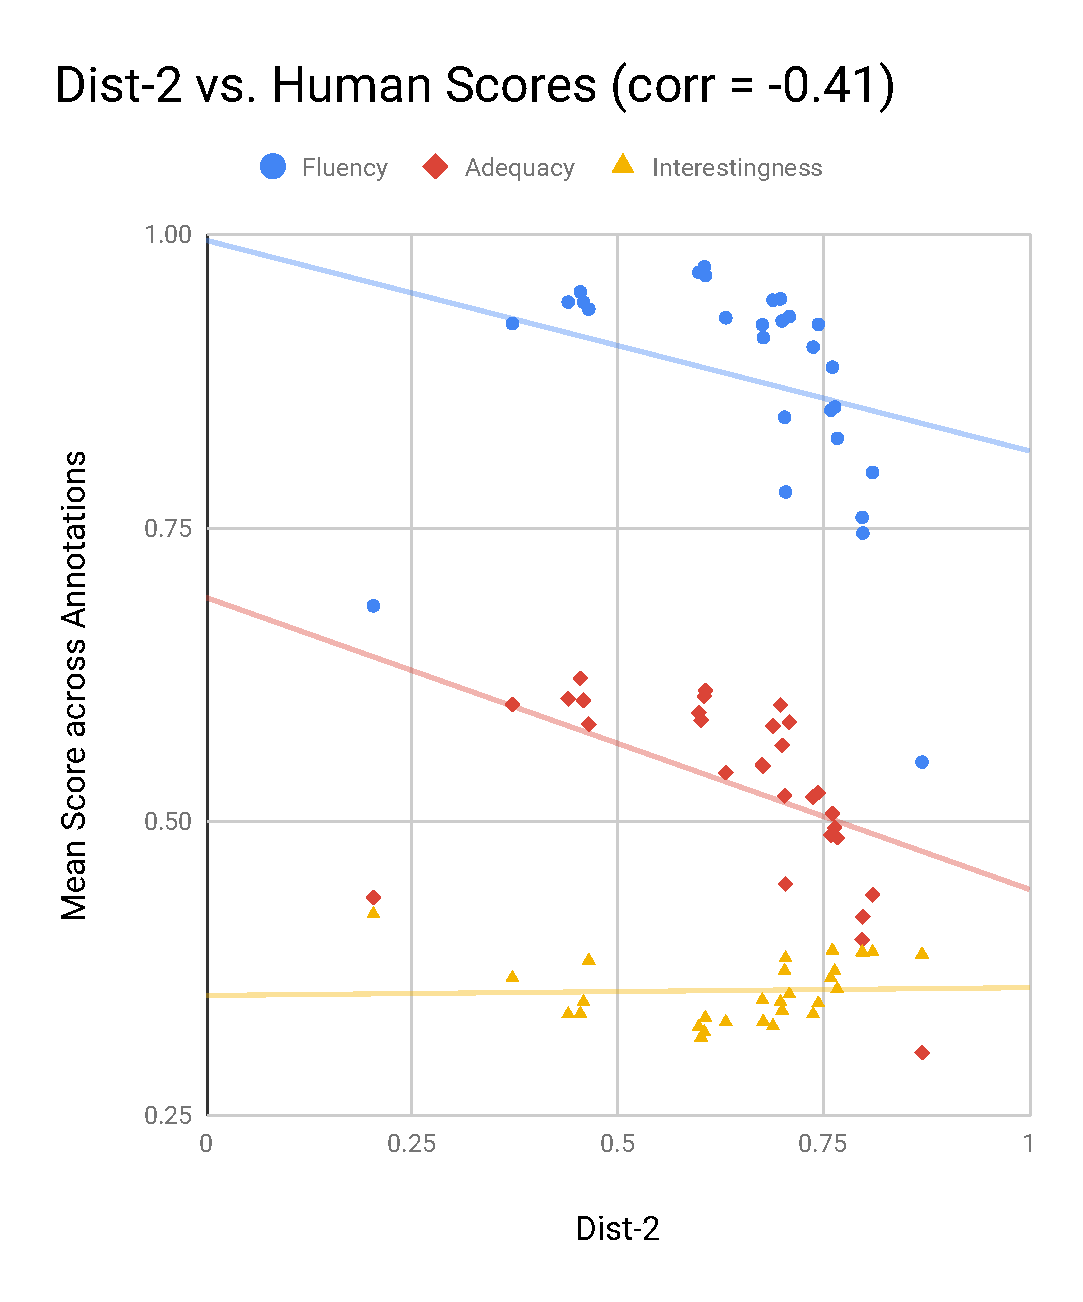
\includegraphics[width=5cm]{figures/dist2_vs_human.pdf}
    \end{subfigure}
    \begin{subfigure}[l]{5cm}
        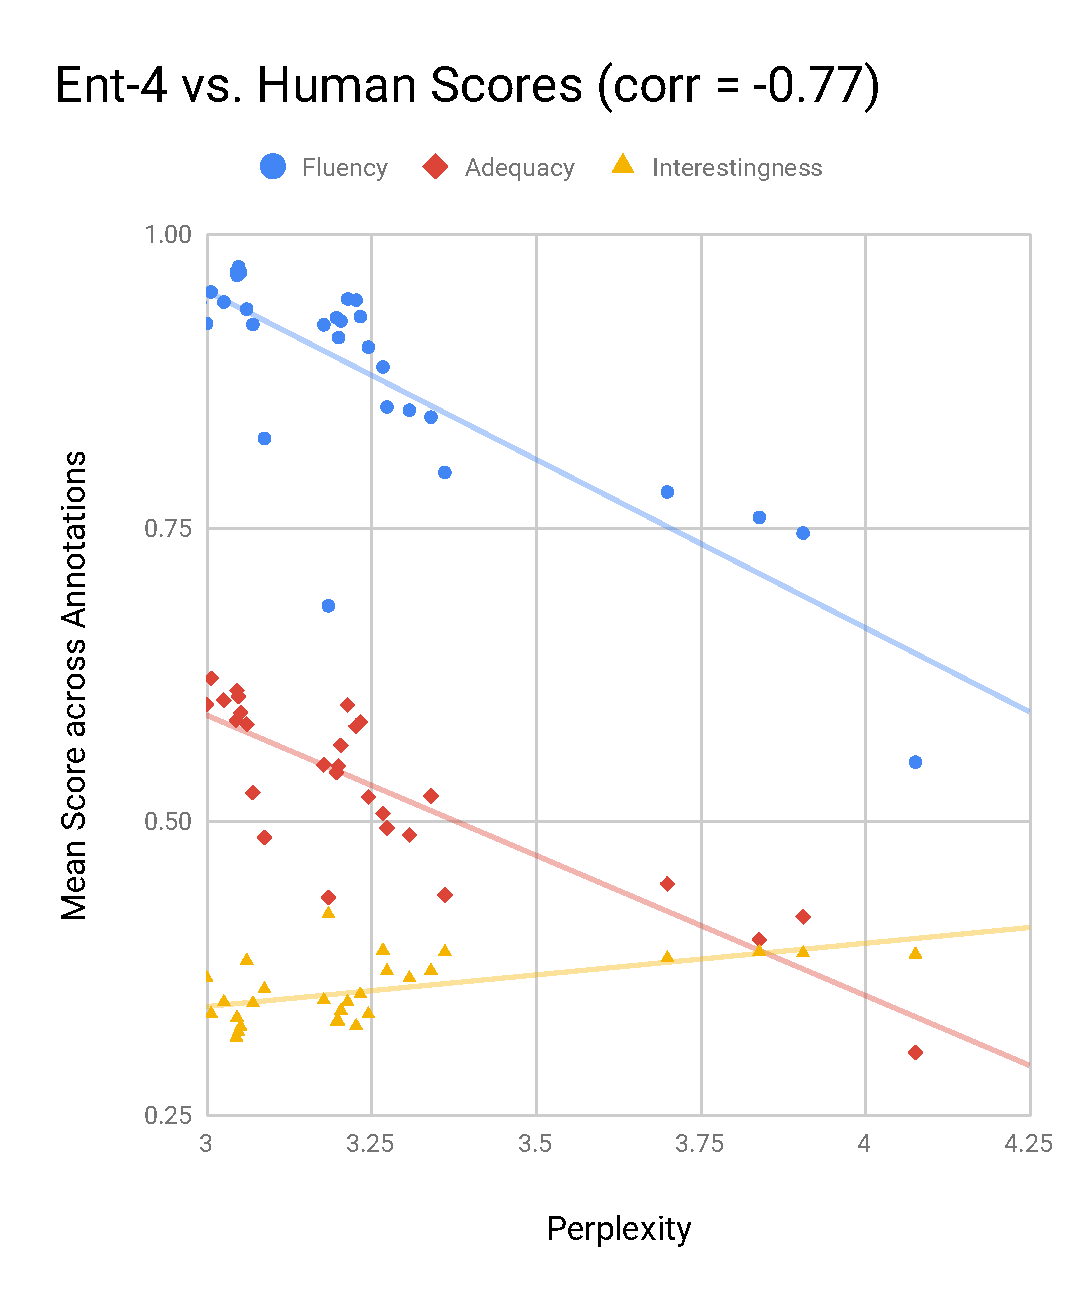
\includegraphics[width=5cm]{figures/ent4_vs_human.pdf}
    \end{subfigure}
    \begin{subfigure}[l]{5cm}
        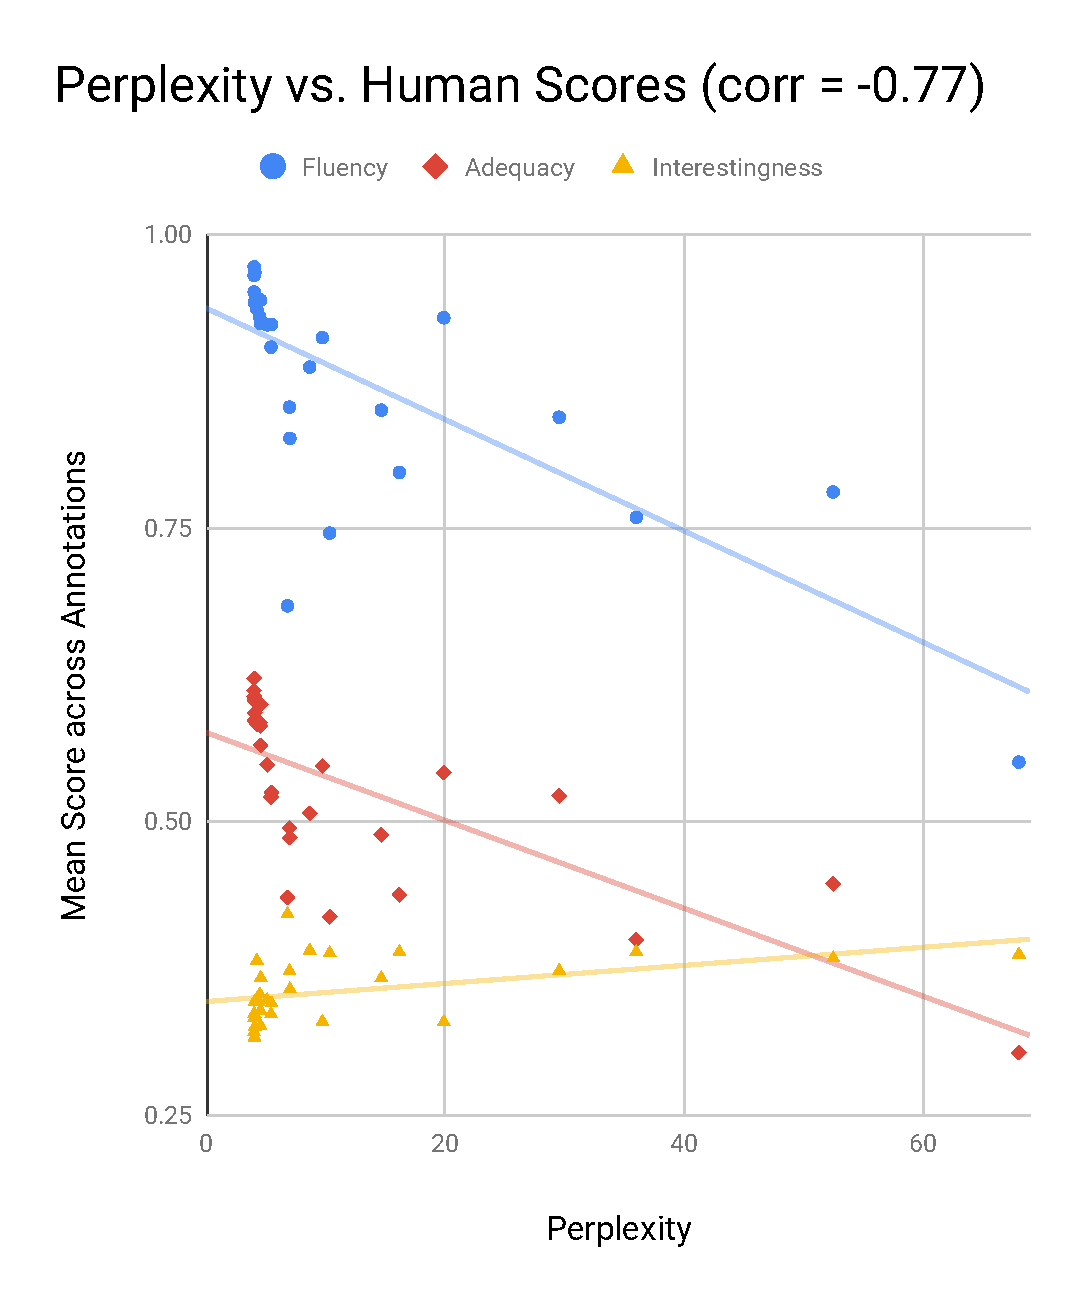
\includegraphics[width=5cm]{figures/perplexity_vs_human.pdf}
    \end{subfigure}
    \caption{Each decoding strategy is plotted, showing that human-perceived quality is negatively correlated with diversity. The Pearson Correlation coefficients between each statistic and the average of fluency, coherence, and interestingness are shown in parentheses.}
    \label{fig:correlations}
\end{figure*}

\begin{table*}[t]
    \centering
    \small
    \begin{tabular}{|l|l|}
    \hline
    \multicolumn{2}{|l|}{\rule{0pt}{0.35cm} \textbf{Prompt:} Look, nobody knows we did it.}  \\ 
    \hline \hline
    \textbf{RS 0.5} &  \textbf{Standard BS} \\
    \hline
\makecell[l]{
I don't know what you're talking about. \\
What's the matter with you? \\
I don't know what it is. \\
I don't think so. \\
He's got to get out of here. \\
}&
\makecell[l]{
We've got to get out of here. \\
What do you mean? \\
I don't think it's a good idea. \\
I don't know what to say. \\
I don't know what's going on. \\
}\\
    \hline
    \hline
    \textbf{RS 1.0} & \textbf{Standard BS with PDC} \\
    \hline
    
\makecell[l]{
I can't find it. \\
They're our ships. \\
It's all right anyone is the right to interfere. \\
We didn't have a plan I engineered a policy. \\
Same time you pick us up at six and get we. \\
}&
\makecell[l]{
I don't know! \\
I don't think so. \\
What do you mean? \\
Why didn't you tell me? \\
That's why we're here. \\
}\\
    \hline
    \hline
    \textbf{RS 1.0,top10} & \textbf{RS 1.0,top10 with PDC} \\
    \hline
\makecell[l]{
I don't know what else to do. \\
It doesn't have to be that way! \\
We're in the air! \\
I've seen a guy in his place in a it. \\
And I'm not we any more. \\
}&
\makecell[l]{
What do you mean? \\
I don't think so. \\
That's why I'm here. \\
It's all right we. \\
We've been through this before. \\
}\\
\hline
\hline


    \textbf{NPAD0.3 BS} & \textbf{Cluster5 BS} \\
    \hline
\makecell[l]{
I don't think it's a good idea. \\
I don't know what to say. \\
I don't know what's going on. \\
I don't know what to do. \\
I don't know what's going on here. \\
}&
\makecell[l]{
I don't know why. \\
What do you mean? \\
I don't think so. \\
How do you know that? \\
I'll tell you what. \\
}\\
\hline
\hline

\textbf{Top3Cap BS} & \\
\hline
\makecell[l]{
We've got to get out of here. \\
What do you mean? \\
I don't think it's a good idea. \\
I don't know what to say. \\
I don't know what's going on. \\
} & \\

\hline
    \end{tabular}
    \caption{Responses to an example prompt for selected methods. More examples can be seen in the appendix.}
    \label{examples}
\end{table*}

\subsubsection{The Quality Diversity Tradeoff}

The goal of diverse decoding strategies is to generate high-quality candidate sequences which span as much of the space of valid outputs as possible. 
However, we find there to be a marked trade-off between diversity and quality.
This can be seen in Figure \ref{fig:correlations}, where we plot the human-judged quality score for each dialog experiment against our primary diversity descriptive statistics.
Fluency and adequacy are both strongly negatively correlated with diversity.
While we had expected interestingness to be positively correlated with diversity, the fact that it is not suggests that existing diversity statistics are insufficient for capturing what it means to humans for outcomes to be interesting.

Likewise, in image captioning, the mean SPICE score of the 10 candidate captions (averaged over all examples for each experimental setting) is strongly anti-correlated with diversity, with a Pearson correlation coefficient of -0.83 with the Ent-4 measure and -0.84 with Dist-2.
Clearly it remains an open challenge to generate a diverse set of image captions that are all high-quality.

When researchers choose to use a diverse decoding strategy, they must decide where on the quality-diversity tradeoff they would like to lie; selecting an optimal method depends strongly on one's tolerance for errors.
In machine translation, where mistakes could severely impact coherence, beam search-based methods, which tend to result in better fluency and coherence, but worse diversity might be preferred.  
In more open-ended applications, where novel text is of greater importance, increased diversity could be worth the fluency and coherency hit.
As state-of-the-art models continue to improve, one would hope that the quality cost of encouraging diversity will continue to decrease. 

In the interest of reporting a single overall best method for each task, we computed a sum-of-ranks score for each method.
For dialog, we ranked the methods each by fluency, coherence, interestingness, and Ent-4, and then took a weighted sum of the four ranks, with 50\% of the weight assigned to Ent-4, and 50\% distributed evenly among the human evaluation ranks.
Overall, clustered beam search and standard BS (beam size 100, PDC) have the best scores, followed by clustered beam search (beam size 10).
Similarly, for image captioning, we rank the methods by their mean SPICE score and by Ent-4.
Summing these ranks, random sampling (temp 1.0, top-10 capping, PDC) came in first.
Standard beam search, Hamming Diversity beam search, and Top-$g$ capping beam search (beam size 10) tied for second.

\subsection{Random Sampling-based Methods}
Higher sampling temperatures result in both an increase in diversity in generated responses and a reduction in overall quality.
In the dialog domain, evaluators consistently rate the responses sampled with temperature 1.0 to have worse fluency, coherence, and interestingness when those sampled with temperature 0.5.
In the image captioning domain, lower temperature improves automatic evaluation metrics for quality while reducing diversity.

For dialog, restricting sampling to the top-10 vocabulary words is a more effective strategy than adjusting temperature for ensuring balance between the quality and diversity of outputs.
Top-10 random sampling has the highest fluency, coherence, and interestingness, as well as significantly lower perplexity than other random sampling methods.
However, this trend did not extend to image captioning, where top-10 random sampling results in both worse SPICE scores and lower diversity measures than setting the temperature to 0.7.
This may be because image captioning is a less ambiguous task than open-ended dialog, leading to a better-trained model that puts more probability mass on high-quality vocabulary words, ameliorating the challenge top-$c$ filtering is designed to eliminate: that of a long tail of low probability vocabulary words taking up a large amount of probability mass.

\subsubsection{Beam Search-based Methods}

For dialog, clustered beam search (Cluster5 BS) performs the best of all beam search methods in terms of human-judged interestingness. It ties for best with NPAD0.3BS on fluency and ties with Standard BS on coherence.
Iterative beam search (Iter5 BS) achieves the greatest diversity, but at the expensive of quality.
It has the lowest human-judged coherence among beam search methods; thus, we do not evaluate this method on image captioning.
For image captioning, Cluster5 BS has the highest diversity among beam search methods, but this difference is quite small.
Cluster5 BS also has the highest SPICE@10 score, indicating it is the best method for generating at least one high quality candidate.
However, Top3Cap BS results in the highest mean SPICE score, suggesting it is best at ensuring all outputs are reasonable quality.
% This indicates that for rereanking tasks 

\subsubsection{Effect of Over-sampling}

In our experiments, we explore over-sampling 100 outputs, and then either using post-decoding clustering (PDC) or re-ranking by log-likelihood to filter these 100 down to 10 diverse outputs.

In the dialog domain, this over-sampling approach is a definite win.
When over-sampling with random sampling both methods of filtering substantially improve human judgements of fluency and adequacy compared to random sampling only 10 outputs.
However, interestingness scores go down, and while the outputs are still more diverse than beam search-based methods, they are less diverse than random sampling without filtering.
In the beam search methods that use a beam size of 100 then filter down to 10, human-judged quality is on par with beam size 10 results, but diversity is considerably higher.

When comparing the two types of filtering, PDC results in higher interestingness and diversity statistics, while log-likelihood re-ranking improves fluency and adequacy.
This again demonstrates the trade-off between quality and diversity.\footnote{In the appendix, we show results with every method where we generate 10 samples; generate 100 samples followed by selecting the 10 most likely outputs; and generate 100 samples followed by post-decoding clustering to select 10 outputs.}

For image captioning, over-sampling with reranking does not consistently improve quality as it does in the dialog domain.
Mean SPICE score is improved for random sampling but not for beam search. 
SPICE@1 becomes worse for both random sampling and decoding, while SPICE@10 improves for random sampling, and for beam search when PDC is applied.
From these results, we can conclude that over-sampling then ranking does not have a sizeable effect, either negative or positive, on quality.
Moreover, the diversity of the captions generated by random sampling actually decreases when oversampling. The diversity of beam search-generated captions does improve with over-sampling.

While oversampling does generally improve outcomes on the diversity/quality tradeoff, it is more computationally expensive, particularly with beam search.
Running PDC also requires generating sentence embeddings for every output, which adds additional computation time.





\section{Impact of Decoding Strategy on the Detection of Machine-Generated Text}
\label{section:detection}


State-of-the-art generative language models are now capable of producing multi-paragraph excerpts that at a surface level are virtually indistinguishable from human-written content \citep{zellers2019defending,radford2019language,adelani2020generating}.
Often, only subtle logical fallacies or idiosyncrasies of language give away the text as machine-generated, errors that require a close reading and/or domain knowledge for humans to detect.

Deceptive text, whether human- or machine-generated, has entered the sphere of public concern \citep{cooke2018fake}.
It propogates quickly \citep{vosoughi2018spread}, sets political agendas \citep{vargo2018agenda}, influences elections \citep{allcott2017social}, and undermines user trust \cite{wang2012serf, song2015crowdtarget}.
Recently, \citet{adelani2020generating} have shown that automatically generated reviews are perceived to be as fluent as human-written ones.
As generative technology matures, authors, well-meaning or otherwise, will increasingly employ it to augment and accelerate their own writing.
% It is more imperative now than ever for both humans and automated systems to be able to detect and identify machine-generated texts in the wild.
However, there has thus been little inquiry into the textual properties that cause humans to give generated text high human-like ratings compared to those that cause automatic systems to rate it highly.

This task of trying to guess whether text is coming from a robot or a fellow human was made famous by the Turing Test \citep{turing1950computing}.
It continues to be used is chatbot evaluation \citep{lowe2017towards}.
The related (but not identical) task of asking human raters to judge the quality of machine-generated excerpts remains the gold-standard for evaluating open-domain generation systems \citep{van2019best}.

In turns out that even with a fixed language model, choice of decoding strategy has a huge impact on the detectability of generated text.
Using top-$k$ random sampling, a decoding method where only the selection of high-likelihood words is permetted, means we are less likely to make a poor choice and create the type of mistakes that are easy for humans to detect.
Since humans are not proficient at identifying when a model subtly favors some utterances more often than a human author would, they don't notice the over-representation of high-likelihood words in the generated text.
In contrast, automatic systems excel at identifying statistical anomalies and struggle to build deeper semantic understanding.
Top-$k$ in particular creates text that is easy for machines to detect but very hard for humans.
Thus, we observe the general trend: as the number of unlikely words available to be chosen is increased, humans get {\em better} at detecting fakes while automatic systems get {\em worse}.

In this work, we study three popular random decoding strategies---top-$k$, nucleus, and temperature sampling---applied to GPT-2 \cite{radford2019language}.
We draw a large number of excerpts generated by each strategy and train a family of BERT-based \cite{devlin2018bert} binary classifiers to label text excerpts as human-written or machine-generated.
We find large differences in human rater and classifier accuracy depending on the decoding strategy employed and length of the generated sequences.
Regardless of strategy, we find human raters achieve significantly lower accuracy than the automatic discriminators.
We also show that when a decoding strategy severely modifies the unigram token distribution, as top-$k$ does, humans have trouble detecting the resultant generated text, but automatic classifiers find it the easiest to discriminate.
Worryingly, we further find that classifiers are brittle; they generalize poorly when trained to discriminate samples from one strategy and then evaluated on samples from another.

\subsection{Detection as a Task}
The rise of machine-generated content has led to the development of automated systems to identify it.
\textsc{Grover} was designed to not only generate convincing news excerpts but to also identify them using a fine-tuned version of the generative model itself \citep{zellers2019defending}.
GLTR, expecting attackers to use sampling methods that favor high-likelihood tokens, aims to make machine-generated text detectable by computing histograms over per-token log likelihoods \citep{gehrmann2019gltr}.
\citet{bakhtin2019real} frame human-text detection as a ranking task and evaluate their models' cross-domain and cross-model generalization, finding significant loss in quality when training on one domain and evaluating on another.
\citet{schuster2019we} argue that the language distributional features implicitly or explicitly employed by these detectors are insufficient; instead, one should look to explicit fact-verification models.
Finally, discriminators for whether text is machine-generated are a promising research  direction in adversarial training \citep{lin2017adversarial,li2017adversarial} and in automatic evaluation of generative model quality \citep{novikova2017we,kannan2017adversarial,lowe2017towards}. 

We frame the detection problem as a binary classification task: given an excerpt of text, label it as either human-written or machine-generated.
In particular, we are interested in how variables such as excerpt length and decoding strategy impact performance on this classification task. 
We thus create several datasets.
Each is approximately balanced between positive examples of machine-generated text and negative examples of human-written text.
While they all share the same human-written examples, each dataset contains a different set of machine-generated examples sampled using one particular decoding strategy.
We also build additional datasets by truncating all of the examples to a particular sequence length,

By training a separate classifier on each dataset, we are able to answer questions about which decoding strategy results in text that is the easiest to automatically disambiguate from human-written text.
We are also able to answer questions about how the length of the examples in the training set impacts our ability to automatically classify excerpts of that same length as either human-written or machine-generated.

\subsection{Method}
\subsubsection{Dataset Construction}
All of our generated text samples are drawn from GPT-2, a state-of-the-art Transformer-based generative language model that was trained on text from popular web pages \citep{radford2019language}.
While we use the GPT-2 \textsc{Large} model with 774M parameters, we found that similar trends to those reported here hold in experiments with smaller language models.

Given an autoregressive language model that defines a probability distribution over the next token given the previous tokens in a sequence, a decoding strategy generates text by deciding how to output a token at each step based on the predicted distributions.
Perhaps the most straightforward decoding strategy is to randomly choose a token with probability proportional to its likelihood.
A challenge with the random sampling approach is that these probability distributions  often contain a long tail of vocabulary items that are individually low-probability but cumulatively comprise a substantial amount of probability mass.
\citet{holtzman2019curious} observe that choosing tokens from this tail often leads to incoherent generations.

Top-$k$ sampling, nucleus sampling, and (in the extreme) beam search have all been proposed to heuristically promote samples with higher per-token likelihoods.
Top-$k$ and nucleus sampling both do so by setting the likelihood of tokens in the tail of the distribution to zero.
Top-$k$ restricts the distribution to all but the $k$ most likely tokens, where $k$ is a constant \citep{fan2018hierarchical}.
Nucleus sampling, also called top-$p$, truncates the distribution at each decoding step $t$ to the $k_t$-most-likely next tokens such that the cumulative likelihood of these tokens is no greater than a constant $p$ \citep{holtzman2019curious}.

We thus consider three different decoding strategy settings:
\begin{itemize}[noitemsep,topsep=0pt]
  \item Sample from the untruncated distribution
  \item Top-$k$, choosing $k$=40 \citep{radford2019language}.
  \item Nucleus sampling (aka top-$p$), choosing $p$=0.96 \citep{zellers2019defending}.
\end{itemize}

In addition, we form ``negative" examples of human-written text by taking excerpts of web text that come from the same distribution as GPT-2's training data.\footnote{\url{https://github.com/openai/gpt-2-output-dataset}}
By picking text that resembles GPT-2's train set, we ensure that our classifiers can't simply take advantage of stylistic differences between the human-written text corpus and the kind of text GPT-2 was trained to generate.

For each decoding method, we construct a training dataset by pairing 250,000 generated samples with 250,000 excerpts of web text.
5,000 additional paired samples are kept aside for validation and test datasets.
Lastly, we filter out excerpts with fewer than 192 WordPiece tokens \citep{wu2016google} (excerpts might be quite short if the model produces an end-of-text token early on). See Appendix~1 for final dataset sizes.

A crucial question when generating text with a language model is whether or not to provide a priming sequence which the language model should continue.
Unconditioned samples, where no priming text is provided, in conjunction with top-$k$ sampling, lead to pathological behavior for discriminators as the first token of the generated text will always be one of $k$ possible options.
On the other hand, if long sequences of human text are used as priming, the space of possible generated sequences is larger, but the detection problem shifts from one of ``how human-like is the generated text?" to ``how well does the generated text follow the priming sequence?".

Since in this study we are interested in the former simpler question, we create two datasets, one with no priming, and one with the minimum amount of priming possible: a single token of web text.
This means that for every excerpt of web text in the training set, there is an excerpt of machine-generated text that starts with the same token.
We find that even with limited priming, the ability of automatic detectors can be strongly impacted.

To study the effect of excerpt length, we construct variations of the above datasets by truncating all excerpts to ten possible lengths ranging from 2 to 192 WordPiece tokens \cite{wu2016google}. In total, we obtain sixty dataset variations: one per sampling method, truncation length, and choice of priming or no priming.

% Table generated by Excel2LaTeX from sheet 'simple_baselines'

\begin{table*}[t]
  \centering
  \small
    \begin{tabular}{|l||cc||cc|cc|cc|c||c|}
    \hline
          & \multicolumn{2}{c||}{BERT} & \multicolumn{2}{c|}{BagOfWords} & \multicolumn{2}{c|}{HistGLTR} & \multicolumn{2}{c|}{Hist50Buckets} & \multicolumn{1}{l||}{TotalProb} & \multicolumn{1}{l|}{Human} \\
    Method & \multicolumn{1}{l}{acc} & \multicolumn{1}{c||}{AUC} & \multicolumn{1}{c}{acc} & \multicolumn{1}{c|}{AUC} & \multicolumn{1}{c}{acc} & \multicolumn{1}{c|}{AUC} & \multicolumn{1}{c}{acc} & \multicolumn{1}{c|}{AUC} & \multicolumn{1}{c||}{acc} & \multicolumn{1}{c|}{acc}\\
    \hline
    k40-1wordcond & 0.88  & 0.99  & 0.79  & 0.87  & 0.52  & 0.52  & 0.69  & 0.76  & 0.61 & 0.64 \\
    p0.96-1wordcond & 0.81  & 0.89  & 0.60  & 0.65  & 0.53  & 0.56  & 0.54  & 0.56  & 0.63 & 0.77 \\
    p1.0-1wordcond & 0.79  & 0.92  & 0.59  & 0.62  & 0.53  & 0.55  & 0.54  & 0.55  & 0.65 & 0.71\\
    % What amount of precision do we want?
    % k40-1wordcond & 0.876 & 0.987 & 0.791 & 0.866 & 0.515 & 0.522 & 0.695 & 0.757 & 0.608 \\
    % p0.96-1wordcond & 0.812 & 0.895 & 0.604 & 0.650 & 0.533 & 0.562 & 0.543 & 0.559 & 0.626 \\
    % p1.0-1wordcond & 0.793 & 0.924 & 0.591 & 0.621 & 0.529 & 0.548 & 0.535 & 0.545 & 0.655  \\
    \hline
    \end{tabular}%
  \caption{Performance (accuracy and AUC) of the fine-tuned BERT classifier and several simple baselines on detecting length-192 sequences generated with one word of priming (1worccond). Note that p1.0 refers to untruncated random sampling, where we sample from 100\% of the probability mass. The last column shows human performance on the same task where accuracy with a 50\% baseline is computed by randomly pairing samples from each decoding strategy with a human-written sample.}
  \label{tab:baselines}%
\end{table*}%

\subsubsection{Methods for Automatic Detection}
The primary discriminator we employ is a fine-tuned BERT classifier \citep{devlin2018bert}.
We fine-tune one instance of BERT per dataset variation described above.
For the longest sequence length, $n$=192, we compare BERT's performance with several simple baselines that have been proposed in other work.

\paragraph{Fine-tuned BERT}
We fine-tune BERT-\textsc{Large} (cased) on the task of labeling a sentence as human- or machine- generated.
The models are trained for 15 epochs, with checkpoints saved every 1000 steps, and a batch size of 256.
All results are reported on the test set using the checkpoint for which validation accuracy was highest.

\paragraph{Bag-of-Words}
% \textsc{BoWDisc} 
For each sequence, we compute a bag-of-words embedding where each dimension corresponds to a token in GPT-2's  50,000 token BPE vocabulary \citep{sennrich2016neural}, and we count how many times that token appears in the text sequence. 
We then train a logistic regression binary classifier to predict human- or machine-written given this 50,000-dimensional embedding.
We experimented with truncating embedding size by removing entries for infrequent vocabulary words, but this did not improve performance.

\paragraph{Histogram-of-Likelihood Ranks}
Following GLTR \citep{gehrmann2019gltr}, we compute the probability distribution of the next word given the previous words in a text sequence according to a trained language model (in our case the same GPT-2 model that was used for generation).
At each sequence position, we rerank the vocabulary words by likelihood, and record the rank of the ground-truth next word within this list.
These ranks are then binned.
GLTR uses four bins, counting (1) the number of times the top 1 word is seen, (2) the number of times words ranked 2 through 5 are seen, (3) words ranked 6-100, and (4) words ranked \textgreater100.
However, we observe higher accuracy when 50 bins are spread uniformly over the possible rankings.
This means that since there are 50,000 vocabulary words, the first bin counts the number of times the actual next word was within the 1,000 mostly likely next words, the second bin counts the 1,001-2,000th, and so on.
We then train logistic regression binary classifiers to predict human- or machine-written given either the 4-dimensional histograms or 50-dimensional histograms as input.

\paragraph{Total Probability}
\citet{solaiman2019release} propose a very simple baseline consisting of a threshold on the total probability of the text sequence.
An excerpt is predicted as machine-generated if its likelihood according to GPT-2 is closer to the mean likelihood over all machine-generated sequences than to the mean of human-written ones.

\subsubsection{Method for Human Detection}
The human evaluation task is framed similarly to the automatic one.
We ask the raters to decide whether a passage of text was written by a human or by a computer algorithm. (Full instructions are in the Appendix.)
Raters are allowed to choose between four options: ``definitely" or ``possibly" machine-generated and  ``definitely" or ``possibly" human-written.
They are first shown an excerpt of length 16 WordPiece tokens.
After they make a guess, the length of the excerpt is doubled, and they are asked the same question again.
This continues until the entire passage of length 192 tokens is shown.
Passages are equally likely to be human-written or machine-generated, with the machine-generated excerpts being evenly split between the three sampling strategies considered in this paper.

Initially, Amazon Mechanical Turk (AMT) raters were employed for this task, but rater accuracy was poor with over 70\% of the ``definitely" votes cast for ``human" despite the classes being balanced.
Accuracy, even for the longest sequences, hovered around 50\%.
The same study was then performed with university students who were first walked through ten examples (see Appendix Table 4) as a group.
Afterward, they were asked to complete the same tasks that had been sent to the AMT workers.
No additional guidance or direction was given to them after the initial walk-through.
We will refer to this group as the ``expert raters."
Among them, 52.1\% of ``definitely" votes were cast for human, and accuracy on the longest excerpt length was over 70\%.

\begin{figure*}[t]
\begin{subfigure}{.495\textwidth}
    \center
    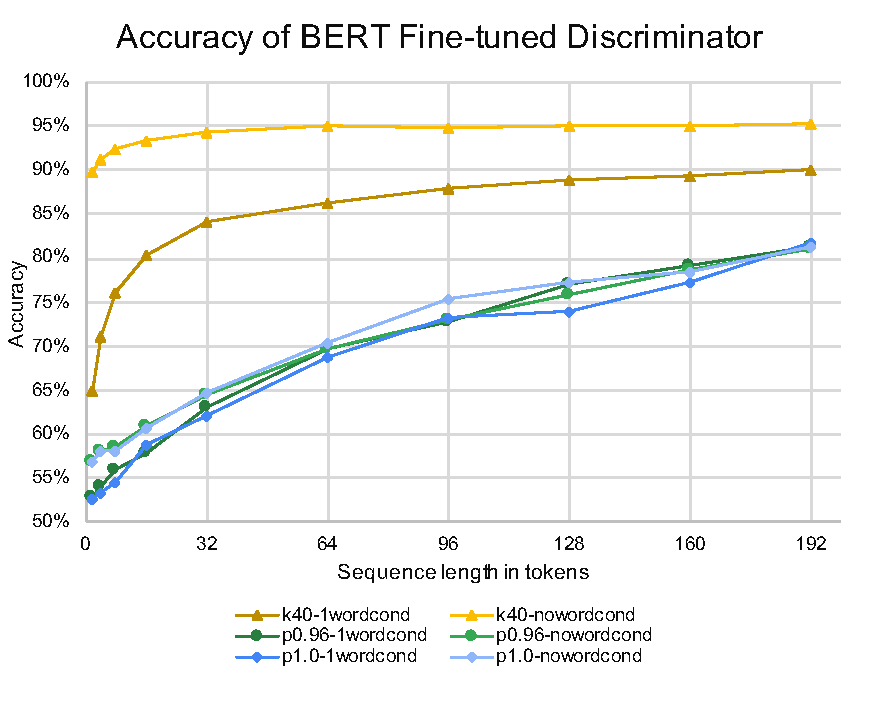
\includegraphics[width=\textwidth]{figures/bert_accuracy}
    \caption{}
    \label{fig:bert_accuracy} 
\end{subfigure}
\begin{subfigure}{.495\textwidth}
    \center
    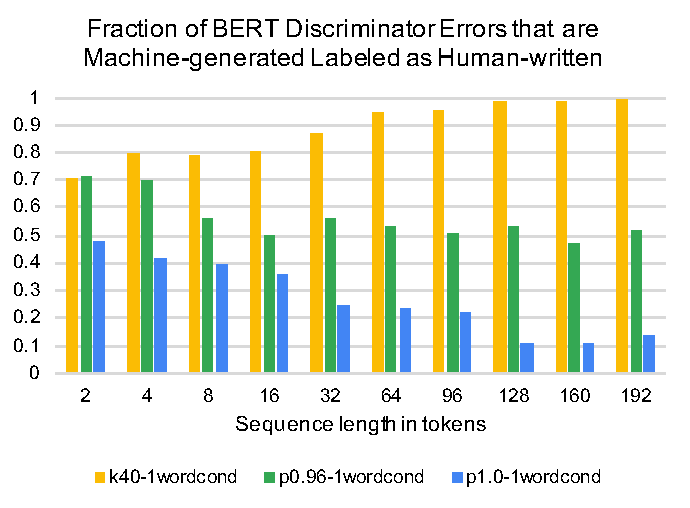
\includegraphics[width=\textwidth]{figures/fraction_incorrect_fp}
    \caption{}
    \label{fig:errors} 
\end{subfigure}
\caption{In \textbf{(a)}, accuracy increases as the length of the sequences used to train the discriminator is increased.
In \textbf{(b)}, we see that the BERT fine-tuned discriminator predicts about the same number of false-positives as false-negatives when trained with samples generated using top-$p$ sampling. However, for top-$k$, it more often mistakes machine-generated text to be human-written, while for untruncated random sampling the opposite is the case.}
\end{figure*}

The human evaluation dataset consisted of 150 excerpts of web text and 50 excerpts each from the three decoding strategies.
Each question was shown to at most three raters, leading to 900 total annotations from the untrained workers and 475 from the expert raters.
A more detailed breakdown can be found in the Appendix.


\subsection{Results}
\label{section:auto_detection}
\paragraph{Simple Baselines}
Table \ref{tab:baselines} shows the performance of the baseline discriminators on length-192 sequences, as compared with fine-tuned BERT.
Reassuringly, BERT far surpasses all simple baselines, indicating that it is not fully possible to solve the detection problem without complex sequence-based understanding.
The simplest baseline, TotalProb, which makes a decision based on the likelihood of the sequence, performs surprisingly well (over 60\% accuracy for all sampling methods) relative to the methods which involve training logistic regression models.

Logistic regression on bag-of-words is the best of the baselines, beating out the histogram-based methods.
While \citet{gehrmann2019gltr} report an AUC of 0.87 on classifying text as real or generated using logistic regression on the four buckets of the GLTR system, we report AUC between 0.52 and 0.56 for this task.
The discrepancy is likely due to the fact that the human-written text in our discriminator training set comes from the same distribution as the text used to train the language model, while in GLTR the human text comes from children's books, scientific abstracts, and newspaper articles. 
The selection of training data for learned detection systems is crucial. In real-world applications, the choice ought to reflect the genres that builders of text-generation systems are trying to impersonate. 

\begin{figure*}[t]
    \begin{subfigure}{.45\textwidth}
        \center
        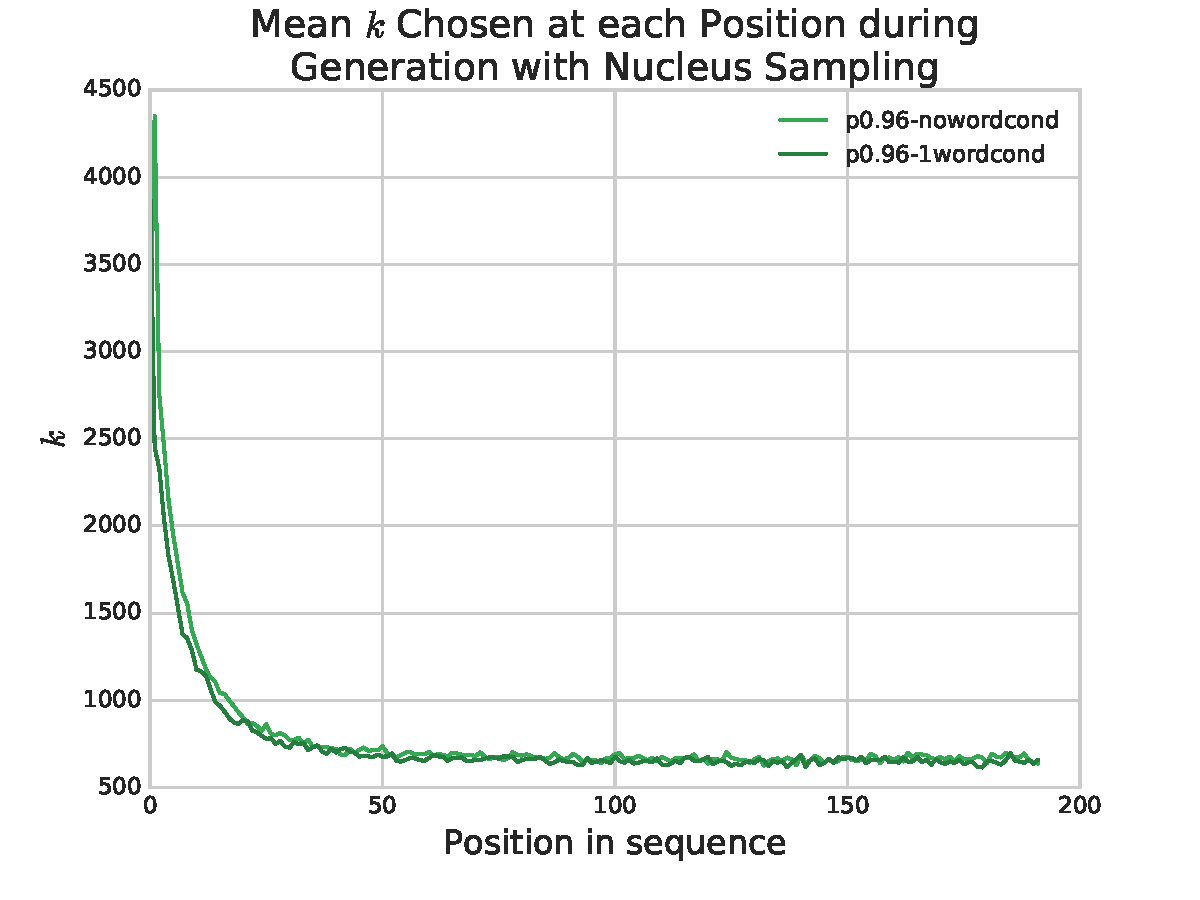
\includegraphics[width=\textwidth]{figures/mean_ks}
        \caption{}
        \label{fig:mean_ks} 
    \end{subfigure}
    \begin{subfigure}{.45\textwidth}
        \center
        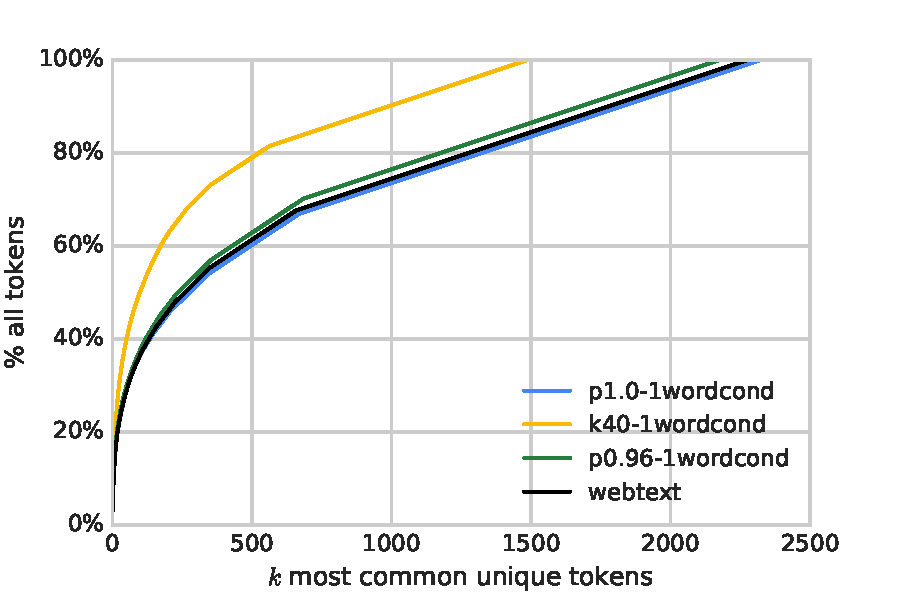
\includegraphics[width=\textwidth]{figures/token_count_histogram}
        \caption{}
        \label{fig:token_count_histogram} 
    \end{subfigure}
    \caption{In \textbf{(a)}, the average (over sequences in the test set) $k$ chosen at each step during generating with nucleus sampling is plotted. Adding a single word of priming strongly impacts the $k$s chosen for the first few positions, but this difference quickly dissipates.
    In \textbf{(b)}, we consider the first token generated in each sequence by top-$k$, and plot what fraction of these are captured by the $k$ most common unique tokens from the vocabulary. Overall, at its first step, top-$k$ concentrates 80\% of its probability mass in the 500 most common tokens from the vocabulary.}
\end{figure*}

\paragraph{Fine-tuned BERT} In Figure~\ref{fig:bert_accuracy}, we begin by observing discriminator accuracy as a function of excerpt length and sampling method.
As can be intuitively expected, as sequence length increases, so too does accuracy.
For unconditioned text decoded with nucleus (p0.96) and untruncated (p1.0) random sampling, we find discriminator accuracy increases from 55\%, near random, to about 81\% for the longest sequences tested.
In contrast, discriminators trained and evaluated on top-$k$ achieve over 80\% accuracy even on 16-token excerpts.

Why are top-$k$'s samples so easy to detect?
In Figure~\ref{fig:token_count_histogram}, we see the percentage of probability mass concentrated in the $k$ most common token types for each sampling method.
While random sampling and nucleus sampling are very similar to human-written texts, we see top-k concentrating up to 80\% of its mass in the first 500 most common tokens.
The other sampling methods as well as human-written texts require at least 1,100 token types for the same.
It is clear that top-$k$'s distribution over unigrams strongly diverges from human-written texts--an easy feature for discriminators to exploit.
In fact, \citet{see2019massively} note that it takes setting $k$ to 1000 to achieve about the same amount of rare word usage and fraction of non-stopword text as as human writing.\footnote{when decoding from the GPT-2 small model with 117M parameters.}
This makes it very easy for the model to pick out machine-generated text based on these distributional differences.

One way to help resolve this problem is to add priming text.
Doing so causes more rare words to be incorporated into the top-$k$ of the unigram distribution.
Adding even a single human word of priming significantly reduces the performance of detectors trained with top-$k$ random sampling.
Without priming, a discriminator trained on sequences of length 2 can classify with $\mathtt{\sim}$90\% accuracy the provenance of the text (Figure \ref{fig:bert_accuracy}).
By adding one priming token, accuracy drops to $\mathtt{\sim}$65\%.
Even on the longest 192-length sequences, top-$k$ discriminator accuracy is 6\% lower on the primed dataset than the unprimed one.

\begin{figure*}[t]
    \centering
    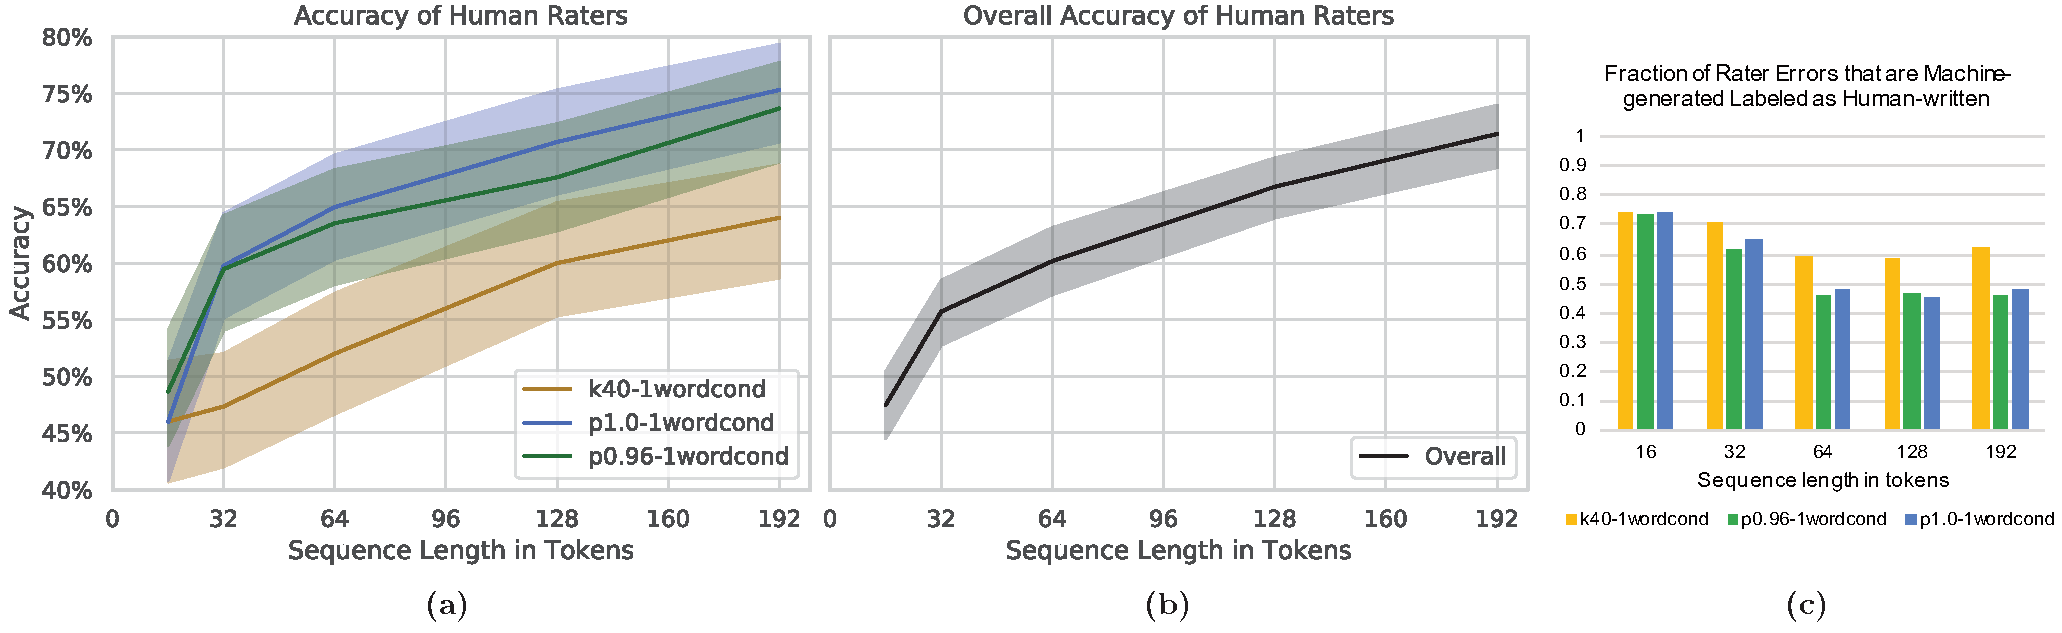
\includegraphics[width=\textwidth]{figures/human_merged}
    \caption{\textbf{(a)} and \textbf{(b)} show human rater accuracy of correctly identifying an excerpt as human-written or machine-written, shown with 80\% confidence internals, in \textbf{(a)}, broken up by decoding strategy and in \textbf{(b)}, overall. Accuracy increases as raters observe more tokens. \textbf{(c)} shows that for short excerpts, most rater mistakes are them incorrectly thinking machine-generated text is human written. The two errors types become more balanced at longer lengths.}
    \label{fig:human_eval} 
\end{figure*}

When generating with nucleus or untruncated random sampling, adding a priming token is not as impactful, as these methods are already sampling from a large fraction (or all) of the probability distribution.
This is seen in Figure \ref{fig:mean_ks} where at the very first step of unprimed generation, nucleus sampling selects from 3075 possible vocabulary words, and at later positions selects from on average more than 500.
Untruncated random sampling always selects from the entire 50,000 word vocabulary, whereas top-$k$ only selects from $k$.


\paragraph{Transferability}
In Table \ref{tab:transfer_accuracy}, we show how discriminators trained with samples from one decoding strategy can transfer at test time to detecting samples generated using a different decoding strategy.
Unsurprisingly a discriminator trained on top-$k$ generalizes poorly to other sampling methods: accuracy drops to as low as 42.5\%, \textit{worse than chance}.
Conversely, training the discriminator with sequences sampled from the untruncated distribution leads to little transferability to detecting top-$k$ samples.
Only the discriminator trained with nucleus sampling (a compromise between unmodified sampling and top-$k$) was able to detect sequences from the other sampling strategies without too much of a hit to accuracy.
As expected, a discriminator trained on an equal portion of data from each decoding method does reasonably at detecting all three.


\begin{table}[t]
  \small
  \centering
  \begin{tabular}{|c c|c|c|c|}
    \hline
    & & \multicolumn{3}{c|}{Eval} \\
    \cline{3-5}
    &            & top-$k$         & nucleus & random \\
    \hline
    \multirow{3}{0.7em}{\rotatebox[origin=c]{90}{\parbox[c]{1cm}{\centering Train}}} 
    & \multicolumn{1}{|c|}{top-k}   & \textbf{90.1} & 57.1          & 43.8 \\
    & \multicolumn{1}{|c|}{nucleus} & 79.1          & \textbf{81.3} & 78.4 \\
    & \multicolumn{1}{|c|}{random}  & 47.8          & 63.7          & \textbf{81.7} \\
    \hline
    & \multicolumn{1}{|c|}{mixed}  & 88.7          & 74.2          & 72.2 \\
    \hline
  \end{tabular}
  \caption{Accuracy of BERT fine-tuned discriminator when trained on samples from one strategy (rows) and evaluated on another (columns). Trained on samples with 192 tokens. The `mixed' dataset is one containing an equal portion of samples from each strategy.}
  \label{tab:transfer_accuracy}
\end{table}

\begin{table}[t]
  \small
  \centering
  %                     p(machine)                              
  % dataset         k0-1wordcond k40-1wordcond p0.96-1wordcond
  % model                                                     
  % k0-1wordcond        0.382658      0.073189        0.226300
  % k40-1wordcond       0.145253      0.608884        0.278946
  % p0.96-1wordcond     0.488926      0.491959        0.517189
  \begin{tabular}{|c c|c|c|c|}
    \hline
    & & \multicolumn{3}{c|}{Eval} \\
    \cline{3-5}
    &            & top-$k$         & nucleus & random \\
    \hline
    \multirow{3}{0.7em}{\rotatebox[origin=c]{90}{\parbox[c]{1cm}{\centering Train}}} 
    & \multicolumn{1}{|c|}{top-k}   & 60.9 & 27.9 & 14.5 \\
    & \multicolumn{1}{|c|}{nucleus} & 49.2 & 51.7 & 48.9 \\
    & \multicolumn{1}{|c|}{random}  &  7.3 & 22.6 & 38.3 \\
    \hline
  \end{tabular}
  \caption{Average probability of `machine-generated' according to each length-192 discriminator. The expected in-domain probability is 0.5. One token of conditioning.}
  \label{tab:transfer-prediction}
\end{table}

Perhaps this lack of transferability is related to each discriminator's calibration.
Indeed, the degree to which a discriminator's average prediction deviates from 50\% is a direct indicator of its accuracy. 
In Table~\ref{tab:transfer-prediction}, we observe that of the three BERT discriminators, only that trained on top-$p$ samples predicts `machine-generated' on approximately 50\% of in-domain examples as expected. 
This same discriminator's behavior holds on datasets generated by other sampling strategies as well. 
In contrast, we observe that discriminators trained on top-k and untruncated random samples severely underestimate the percentage of machine-generated excerpts in out-of-domain datasets.
Even within domain (Figure~\ref{fig:errors}), we find both discriminators heavily favor a single class, increasingly so as the number of tokens increases.

% False-negative = machine-written labeled as human-written
% Negative = machine-written
% Positive = human-written

\begin{table*}
\setlength\tabcolsep{4.5pt}
    \small
    \centering
    \begin{tabular}{|p{0.40in}|p{0.42in}|p{0.35in}|p{0.35in}|p{0.35in}r|p{0.40in}|p{0.42in}|p{0.35in}|p{0.35in}|p{0.35in}r|}
\hline
\textbf{Truth} & \textbf{Raters} & \textbf{p1.0} & \textbf{k40} & \textbf{p0.96} & &
\textbf{Truth} & \textbf{Raters} & \textbf{p1.0} & \textbf{k40} & \textbf{p0.96} & \\
\hline
H & M & H & H & M & &
H & H & M & M & M & \\
\multicolumn{6}{|p{2.88in}|}{
\tiny
EDIT:OKAY!, I guess that'll work for now. \textgreater\_ http://www.teamfortress.com/ and then go buy the game and experience some of the best online gaming I have ever played. \textasciicircum\_\_\textasciicircum Both girls had a really fun time and I had a GREAT time making both of these costumes. Everything was altered even a little bit(dying the pants a darker grey and painting the boots and shirts) But my piece de resistance would have to be my eldest's Medi-Gun.If you have any questions about the costumes, I would be happy to assist you!Oh and here's a video of my daughter before the costume was completed.Thanks!
}&
\multicolumn{6}{p{3.03in}|}{
\tiny
Image copyright Getty Images Image caption Women mourn over the coffin of one of the victim's of Sunday's bombing in Ankara \textparagraph Who'd be in Turkey's shoes right now? \textparagraph Since July last year, hundreds of soldiers and civilians have been killed in terrorist attacks. Suicide bombs have torn into crowds of demonstrators and tourists. Military convoys have been targeted in the heart of the capital. \textparagraph A long-running Kurdish insurgency, once thought to be close to resolution after years of painstaking efforts to build bridges, has erupted once more. \textparagraph The country is awash with Syrian and other refugees. The government has been under pressure to stop them moving on into Europe and prevent would-be jihadis travelling the other way. \textparagraph How dangerous is Turkey's unrest? \textparagraph Tears and destruction amid PKK crackdown \textparagraph Turkey v Islamic State v the Kurds
}\\
\hline
\hline
\textbf{Truth} & \textbf{Raters} & \textbf{p1.0} & \textbf{k40} & \textbf{p0.96} & &
\textbf{Truth} & \textbf{Raters} & \textbf{p1.0} & \textbf{k40} & \textbf{p0.96} & \\
\hline
        M & M & H & - & - & &
        M & M & - & - & H & \\
\multicolumn{6}{|p{2.88in}|}{
\tiny
First off, this thread has done a pretty good job of describing in detail yet another broken touchscreen. That's the difference between a smartphone and a PC with no prying eyes having to snap shots for the police to find. \textparagraph What I would like to address is the mindset that generally surrounds Chrome OS users. To me this is analogous to saying that Apple does``hate their Windows", or that HP does``hate their Macs" as if http://twitter.com/) (and that quote is from two years ago), that anyone who covers smartphones and tablets from a ``PC" perspective is just jealous. \textparagraph Chrome OS is for browsing the web, PC processors can do stronger things in that regard, Windows is a juggernaut on those fronts. This is how I see it. Yes, it can be slow. And yes, you need a fast CPU
}
&
\multicolumn{6}{p{3.03in}|}{
\tiny
FOR ALABAMA, GOOD WEEKS \textparagraph AND A TOUR OF CAIRO \textparagraph THE ALABAMA COMMITTEE ON THE STUDY OF THE AMERICAN SECURITY AGENDA, \textparagraph America's future has been mapped out in carved stone. Metro Atlanta's last US congressman, Bill Posey, was a inextricable integral element of the Citadel project as it became another metaphor for Atlanta's transformation from an industry backwater into the finance and information hub of the nation's capital. Meanwhile, Cobb County -- Atlanta's geode of change -- is home to some of the largest industrial parks in the South, a regional cultural center, a 100-year-old manufacturing town and a potent symbol of the former city's cherished Georgian past. The gentry still live there, the defunct industrial landscapes carry the names of
}\\
\hline
\hline
\textbf{Truth} & \textbf{Raters} & \textbf{p1.0} & \textbf{k40} & \textbf{p0.96} & &
\textbf{Truth} & \textbf{Raters} & \textbf{p1.0} & \textbf{k40} & \textbf{p0.96} & \\
\hline
        M & H & - & - & M & &
        M & H & - & M & - & \\
\multicolumn{6}{|p{2.88in}|}{
\tiny
Exidentia at Eurnari, is an upcoming Cryptopia event which is currently still in development. Be a part of the first live stream of this year's event on 15-16 January 2016! \textparagraph Since the release of v1.22, Exidentia has received a fair amount of user feedback. This event takes place in the underwater Cryptopia they have built. During this event, you will learn about the ocean and areas around it, and be reached by a treasure hunter that helps you explore the different areas. \textparagraph There will be six different levels in this event that you will become acquainted with: thought Polar Lava, Ocean Seared Cones and Celestine Floors, Sea Damaged Aerie Bricks, coast Puddle (congipit stopping at red water), Shaikh Swamp and Bugmite. At rotating points, you will learn how to access various types of creatures
}
&
\multicolumn{6}{p{3.03in}|}{
\tiny
Ever since the opening of the North American College of Art Education in 1990, the demand for art education in America has grown steadily, and in recent years we have seen the rise of students that pursue art education not in the classroom but at art academies. This year saw another 50 percent increase in the number of art academies in the United States offering courses -- with an additional 10 percent of students in 2017 taking art. \textparagraph Some major changes have occurred in recent years with regard to the art curriculum and the way students learn, and we will explore each of these in coming months as we look at the various forms of art education. There is no one-size-fits-all approach for this or any other field of study, and students who begin a course in art education may change their plans based on what they see that course, including what lessons they have completed and the resources available, to create meaningful experiences of artistic creation. \textparagraph One important area
}\\
\hline

    \end{tabular}
    \caption{Some 192-token examples where at least two expert raters agreed with each other, but were not in agreement with the automatic discriminators. The first row shows examples where the ground-truth was human-written, the second shows machine-generated examples where the corresponding discriminator guessed incorrectly, and the third shows machine-generated examples where the discriminator was correct, but raters got it wrong.}
    \label{tab:qual_examples}
\end{table*}

\paragraph{Human Evaluation}
Overall human performance across all sampling methods is shown in Figure \ref{fig:human_eval}b.
Even with the multi-paragraph 192-length excerpts, human performance is only at 71.4\%, indicating that even trained humans struggle to correctly identify machine-generated text over a quarter a time.
However, it is worth noting that our best raters achieved accuracy of 85\% or higher, suggesting that it is possible for humans to do very well at this task.
Further investigation is needed into how educational background, comfort with English, participation in more extensive training, and other factors can impact rater performance.

To break up the accuracies by sampling method in a way that is comparable to the results shown for the automatic discriminators, we pair each machine-generated example with a randomly selected one of webtext to create a balanced dataset for each sampling strategy.
Performance is shown in Figure \ref{fig:human_eval}a.
Top-$k$ produces the text that is hardest for raters to correctly distinguish, but as shown in Section \ref{section:auto_detection}, it is the easiest for our automatic detection systems.
Samples from untruncated random sampling and nucleus sampling with $p$=0.96 are equivalently difficult for raters to classify as machine-generated.
Our human evaluation results suggest that much lower $p$-values than the 0.92 to 0.98 range proposed in \citet{zellers2019defending} might be necessary in order to generate text that is considered significantly more human-like to human raters than the text produced by using the untruncated distribution.

Table \ref{tab:qual_examples} gives several examples where human raters and our BERT-based discriminators disagreed.
When raters incorrectly labeled human-written text as machine-generated, often the excerpts contained formatting failures introduced when the HTML was stripped out.
In the middle two examples, topic drift and falsehoods such as Atlanta being the ``information hub of the nation's capital" allowed humans to correctly detect the generated content.
However, in the bottom two examples, the high level of fluency left human raters fooled.

Overall we find that human raters---even ``expert" trained ones---have consistently worse accuracy than automatic discriminators for all decoding methods and excerpt lengths.
In our experiments, randomly-selected pairs of raters agree with each other on a mere 59\% of excerpts on average. (In comparison, raters and discriminators agree on 61\% to 70\% of excerpts depending on the discriminator considered).
We surmise that the gap between human and machine performance will only grow as researchers inevitably train bigger, better  detection models on larger amounts of training data.
While improved detection models are inevitible, it is unclear how to go about improving human performance.
GLTR proposes providing visual aids to humans to improve their performance at detecting generated-text, but it is unlikely that their histogram-based color-coding will continue to be effective as generative methods get better at producing high-quality text that lacks statistical anomalies.

\subsection{Conclusion}
In this work, we study the behavior of automated discriminators and their ability to identify machine-generated and human-written texts. 
We train these discriminators on balanced binary classification datasets where all machine-generated excerpts are drawn from the same generative model but with different decoding strategies.
We find that, in general, discriminators transfer poorly between decoding strategies, but that training on a mix of data from methods can help.
We also show the rate at which discriminator accuracy increases as excerpts are lengthened.

We further study the ability of expert human raters to perform the same task.
We find that rater accuracy varies wildly, but has a median of 74\%, which is less than the accuracy of our best-performing discriminator.
Most interestingly, we find that human raters and discriminators make decisions based on different qualities, with humans more easily noticing semantic errors and discriminators picking up on statistical artifacts.
In our experiments, these artifacts are most prominent with top-$k$ sampling.
However, any strategy that over-samples high-likelihood words is susceptible.
As the $p$ in nucleus sampling is set increasingly lower to achieve more fluent text (some systems are already using $p$ as low as 0.5 \citep{miculicich2019selecting}), the distributional deviations that plague top-$k$ text will surface in nucleus sampling as well.

\citet{holtzman2019curious} explain how a unique attribute of human language is that it dips in and out of low probability zones.
This variance in likelihood is what makes human-written text interesting and exciting to read.
Today's generation systems have not yet solved the problem of mimicking the human cadence without introducing poor word choices that are easy for humans to detect. 
Generation systems often optimize for fooling humans without acknowledging the trade-off that exists between human perception of quality and ease of automatic detection.
We therefore suggest three prongs for future research:

\begin{enumerate}[noitemsep,topsep=0pt]
    \item Identifying ways to improve the language models and decoding strategies we use in order to generate text that is both exciting (ie. unlikely) and semantically plausible.
    
    \item Building better world understanding into automatic discriminators so that they are more capable of detecting the types of errors that humans notice.

    \item Developing tools and educational materials to improve humans' ability to detect machine-generated text. These may include automatic detectors with components that explain their predictions.

\end{enumerate}

Finally, we would like to note that all of our experiments were performed with English language models, and it remains an open question how the trade-off between ease of human detection and ease of automatic detection might differ for languages that are very different from English. 





\section{Detecting the Boundary between Human-Written and Machine-Generated Text}
\label{section:roft}
